\noindent

\includegraphics[height=1.25cm]{images/pictograms/replication}

\includegraphics[height=1.25cm]{images/pictograms/benchmark}

\includegraphics[height=1.25cm]{images/pictograms/under_construction}

\includegraphics[height=1.25cm]{images/pictograms/FEM}

\includegraphics[height=1.25cm]{images/pictograms/paraview}

%%%%%%%%%%%%%%%%%%%%%%%%%%%%%%%%%%%%%%%%%%%%%%%%%%%%%%%%%%%%%%%%%%%%%%%%%%%%%%%%%%%%%%%%%%%%%%%%%%%

\begin{flushright} {\tiny {\color{gray} \tt python\_codes/fieldstone\_161/text.tex}} \end{flushright}

%\lstinputlisting[language=bash,basicstyle=\small]{python_codes/template_keywords.key}

\par\noindent\rule{\textwidth}{0.4pt}

\begin{center}
\inpython
{\small Code: \url{https://github.com/cedrict/fieldstone/tree/master/python_codes/fieldstone_161}}
\end{center}

\par\noindent\rule{\textwidth}{0.4pt}

%%%%%%%%%%%%%%%%%%%%%%%%%%%%%%%%%%%%%%%%%%%%%%%%%%%%%%%%%%%%%%%%%%%%%%%%%%%%%%%%%%%%%%%%%%%%%%%%%%%

We here consider the $Q_{2,1}\times Q_{1,2} \times Q_{1}'$ element introduced 
by \textcite{huzh11} (2011) which follows \textcite{zhan09} (2009).
The shape functions in 2D are in derived in Section~\ref{MMM-ss:qqq_elt}.

The question we wish to answer is whether this element could be used 
in the context of computational geodynamics. 
The element has been proven stable and verified on a simple 
isoviscous manfufactured solution with trivial boundary conditions,
but quid of more complex boundary conditions ? free surface ? 
sharp viscosity transitions?  buoyancy-driven flow? 


The list of velocity degrees of freedom per element is as follows:
\[
\vec{\cal V} = (u_1,v_1,u_2,v_2,u_3,v_3,u_4,v_4,u_5,v_5,u_6,v_6)
\]
where $u$ is the $x$-component of the velocity field and $v$ its $y$-component,
with the following internal numbering
\begin{verbatim}
u dofs      v dofs

4--6--3     4-----3
|     |     |     |
|     |     5     6
|     |     |     |
1--5--2     1-----2
\end{verbatim}

Remark: the location of the 'extra' 
nodes for u and v are opposite of those for the Fortin $Q_1^+\times P_0$ element, see
Section \ref{MMM-ss:Q1pP02D} (see also \stone~80).

We start with a simple $4\times 3$ element mesh.
$u$ dofs are represented in red and $v$ dofs are shown in blue:


\begin{center}
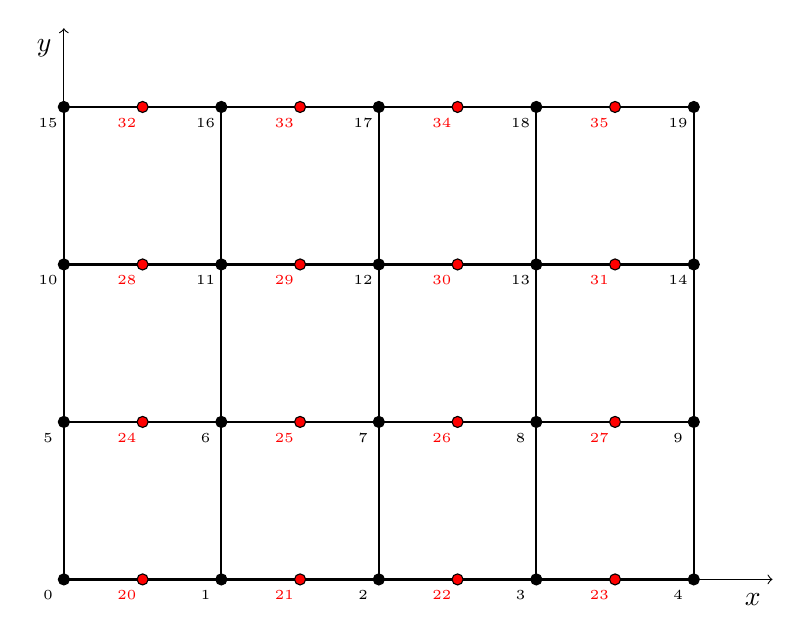
\begin{tikzpicture}
%\draw[fill=gray!23,gray!23](0,0) rectangle (10,8);
%\draw[step=0.5cm,gray,very thin] (0,0) grid (10,8); %background grid

\draw[thick] (1,1) -- (9,1) ;
\draw[thick] (1,3) -- (9,3) ;
\draw[thick] (1,5) -- (9,5) ;
\draw[thick] (1,7) -- (9,7) ;

\draw[thick] (1,1) -- (1,7) ;
\draw[thick] (3,1) -- (3,7) ;
\draw[thick] (5,1) -- (5,7) ;
\draw[thick] (7,1) -- (7,7) ;
\draw[thick] (9,1) -- (9,7) ;

\draw[black,fill=black] (1,1)   circle (2pt);
\draw[black,fill=black] (3,1)   circle (2pt);
\draw[black,fill=black] (5,1)   circle (2pt);
\draw[black,fill=black] (7,1)   circle (2pt);
\draw[black,fill=black] (9,1)   circle (2pt);

\draw[black,fill=black] (1,3)   circle (2pt);
\draw[black,fill=black] (3,3)   circle (2pt);
\draw[black,fill=black] (5,3)   circle (2pt);
\draw[black,fill=black] (7,3)   circle (2pt);
\draw[black,fill=black] (9,3)   circle (2pt);

\draw[black,fill=black] (1,5)   circle (2pt);
\draw[black,fill=black] (3,5)   circle (2pt);
\draw[black,fill=black] (5,5)   circle (2pt);
\draw[black,fill=black] (7,5)   circle (2pt);
\draw[black,fill=black] (9,5)   circle (2pt);

\draw[black,fill=black] (1,7)   circle (2pt);
\draw[black,fill=black] (3,7)   circle (2pt);
\draw[black,fill=black] (5,7)   circle (2pt);
\draw[black,fill=black] (7,7)   circle (2pt);
\draw[black,fill=black] (9,7)   circle (2pt);

\draw[black,fill=red] (2,1) circle (2pt); 
\draw[black,fill=red] (4,1) circle (2pt); 
\draw[black,fill=red] (6,1) circle (2pt); 
\draw[black,fill=red] (8,1) circle (2pt); 

\draw[black,fill=red] (2,3) circle (2pt); 
\draw[black,fill=red] (4,3) circle (2pt); 
\draw[black,fill=red] (6,3) circle (2pt); 
\draw[black,fill=red] (8,3) circle (2pt); 

\draw[black,fill=red] (2,5) circle (2pt); 
\draw[black,fill=red] (4,5) circle (2pt); 
\draw[black,fill=red] (6,5) circle (2pt); 
\draw[black,fill=red] (8,5) circle (2pt); 

\draw[black,fill=red] (2,7) circle (2pt); 
\draw[black,fill=red] (4,7) circle (2pt); 
\draw[black,fill=red] (6,7) circle (2pt); 
\draw[black,fill=red] (8,7) circle (2pt); 

\draw[thin,->] (9,1) -- (10,1); %x
\draw[thin,->] (1,7) -- (1,8); %y
\node[] at (9.75,0.75) {$x$};
\node[] at (0.75,7.75) {$y$};

\node[] at (0.8,0.8) {\tiny 0};
\node[] at (2.8,0.8) {\tiny 1};
\node[] at (4.8,0.8) {\tiny 2};
\node[] at (6.8,0.8) {\tiny 3};
\node[] at (8.8,0.8) {\tiny 4};
\node[] at (0.8,2.8) {\tiny 5};
\node[] at (2.8,2.8) {\tiny 6};
\node[] at (4.8,2.8) {\tiny 7};
\node[] at (6.8,2.8) {\tiny 8};
\node[] at (8.8,2.8) {\tiny 9};
\node[] at (0.8,4.8) {\tiny 10};
\node[] at (2.8,4.8) {\tiny 11};
\node[] at (4.8,4.8) {\tiny 12};
\node[] at (6.8,4.8) {\tiny 13};
\node[] at (8.8,4.8) {\tiny 14};
\node[] at (0.8,6.8) {\tiny 15};
\node[] at (2.8,6.8) {\tiny 16};
\node[] at (4.8,6.8) {\tiny 17};
\node[] at (6.8,6.8) {\tiny 18};
\node[] at (8.8,6.8) {\tiny 19};

\node[] at (1.8,0.8) {\tiny \color{red} 20};
\node[] at (3.8,0.8) {\tiny \color{red} 21};
\node[] at (5.8,0.8) {\tiny \color{red} 22};
\node[] at (7.8,0.8) {\tiny \color{red} 23};

\node[] at (1.8,2.8) {\tiny \color{red} 24};
\node[] at (3.8,2.8) {\tiny \color{red} 25};
\node[] at (5.8,2.8) {\tiny \color{red} 26};
\node[] at (7.8,2.8) {\tiny \color{red} 27};

\node[] at (1.8,4.8) {\tiny \color{red} 28};
\node[] at (3.8,4.8) {\tiny \color{red} 29};
\node[] at (5.8,4.8) {\tiny \color{red} 30};
\node[] at (7.8,4.8) {\tiny \color{red} 31};

\node[] at (1.8,6.8) {\tiny \color{red} 32};
\node[] at (3.8,6.8) {\tiny \color{red} 33};
\node[] at (5.8,6.8) {\tiny \color{red} 34};
\node[] at (7.8,6.8) {\tiny \color{red} 35};

\end{tikzpicture}
\end{center}









\begin{center}
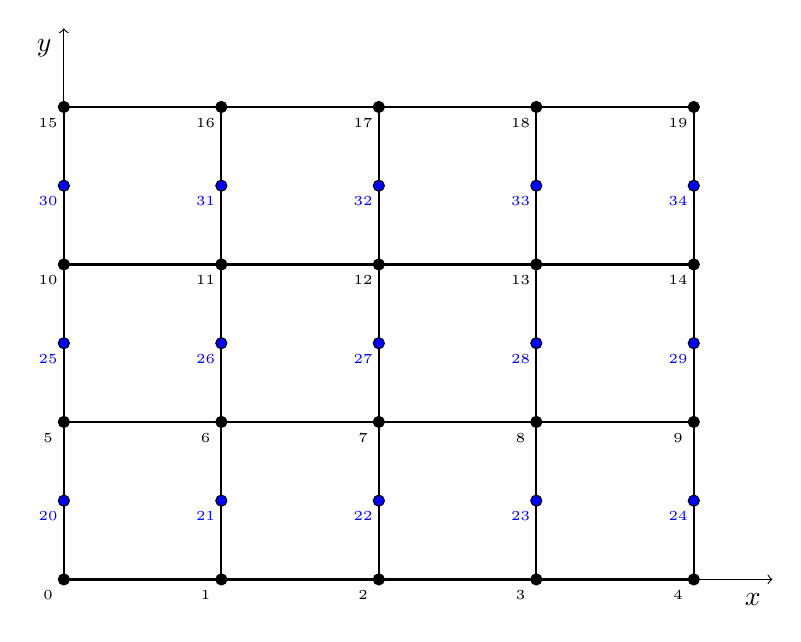
\begin{tikzpicture}
%\draw[fill=gray!23,gray!23](0,0) rectangle (10,8);
%\draw[step=0.5cm,gray,very thin] (0,0) grid (10,8); %background grid

\draw[thick] (1,1) -- (9,1) ;
\draw[thick] (1,3) -- (9,3) ;
\draw[thick] (1,5) -- (9,5) ;
\draw[thick] (1,7) -- (9,7) ;

\draw[thick] (1,1) -- (1,7) ;
\draw[thick] (3,1) -- (3,7) ;
\draw[thick] (5,1) -- (5,7) ;
\draw[thick] (7,1) -- (7,7) ;
\draw[thick] (9,1) -- (9,7) ;

\draw[black,fill=black] (1,1)   circle (2pt);
\draw[black,fill=black] (3,1)   circle (2pt);
\draw[black,fill=black] (5,1)   circle (2pt);
\draw[black,fill=black] (7,1)   circle (2pt);
\draw[black,fill=black] (9,1)   circle (2pt);

\draw[black,fill=black] (1,3)   circle (2pt);
\draw[black,fill=black] (3,3)   circle (2pt);
\draw[black,fill=black] (5,3)   circle (2pt);
\draw[black,fill=black] (7,3)   circle (2pt);
\draw[black,fill=black] (9,3)   circle (2pt);

\draw[black,fill=black] (1,5)   circle (2pt);
\draw[black,fill=black] (3,5)   circle (2pt);
\draw[black,fill=black] (5,5)   circle (2pt);
\draw[black,fill=black] (7,5)   circle (2pt);
\draw[black,fill=black] (9,5)   circle (2pt);

\draw[black,fill=black] (1,7)   circle (2pt);
\draw[black,fill=black] (3,7)   circle (2pt);
\draw[black,fill=black] (5,7)   circle (2pt);
\draw[black,fill=black] (7,7)   circle (2pt);
\draw[black,fill=black] (9,7)   circle (2pt);

\draw[black,fill=blue] (1,2) circle (2pt); 
\draw[black,fill=blue] (3,2) circle (2pt); 
\draw[black,fill=blue] (5,2) circle (2pt); 
\draw[black,fill=blue] (7,2) circle (2pt); 
\draw[black,fill=blue] (9,2) circle (2pt); 

\draw[black,fill=blue] (1,4) circle (2pt); 
\draw[black,fill=blue] (3,4) circle (2pt); 
\draw[black,fill=blue] (5,4) circle (2pt); 
\draw[black,fill=blue] (7,4) circle (2pt); 
\draw[black,fill=blue] (9,4) circle (2pt); 

\draw[black,fill=blue] (1,6) circle (2pt); 
\draw[black,fill=blue] (3,6) circle (2pt); 
\draw[black,fill=blue] (5,6) circle (2pt); 
\draw[black,fill=blue] (7,6) circle (2pt); 
\draw[black,fill=blue] (9,6) circle (2pt); 


\draw[thin,->] (9,1) -- (10,1); %x
\draw[thin,->] (1,7) -- (1,8); %y
\node[] at (9.75,0.75) {$x$};
\node[] at (0.75,7.75) {$y$};

\node[] at (0.8,0.8) {\tiny 0};
\node[] at (2.8,0.8) {\tiny 1};
\node[] at (4.8,0.8) {\tiny 2};
\node[] at (6.8,0.8) {\tiny 3};
\node[] at (8.8,0.8) {\tiny 4};
\node[] at (0.8,2.8) {\tiny 5};
\node[] at (2.8,2.8) {\tiny 6};
\node[] at (4.8,2.8) {\tiny 7};
\node[] at (6.8,2.8) {\tiny 8};
\node[] at (8.8,2.8) {\tiny 9};
\node[] at (0.8,4.8) {\tiny 10};
\node[] at (2.8,4.8) {\tiny 11};
\node[] at (4.8,4.8) {\tiny 12};
\node[] at (6.8,4.8) {\tiny 13};
\node[] at (8.8,4.8) {\tiny 14};
\node[] at (0.8,6.8) {\tiny 15};
\node[] at (2.8,6.8) {\tiny 16};
\node[] at (4.8,6.8) {\tiny 17};
\node[] at (6.8,6.8) {\tiny 18};
\node[] at (8.8,6.8) {\tiny 19};

\node[] at (0.8,1.8) {\tiny \color{blue} 20};
\node[] at (2.8,1.8) {\tiny \color{blue} 21};
\node[] at (4.8,1.8) {\tiny \color{blue} 22};
\node[] at (6.8,1.8) {\tiny \color{blue} 23};
\node[] at (8.8,1.8) {\tiny \color{blue} 24};

\node[] at (0.8,3.8) {\tiny \color{blue} 25};
\node[] at (2.8,3.8) {\tiny \color{blue} 26};
\node[] at (4.8,3.8) {\tiny \color{blue} 27};
\node[] at (6.8,3.8) {\tiny \color{blue} 28};
\node[] at (8.8,3.8) {\tiny \color{blue} 29};

\node[] at (0.8,5.8) {\tiny \color{blue} 30};
\node[] at (2.8,5.8) {\tiny \color{blue} 31};
\node[] at (4.8,5.8) {\tiny \color{blue} 32};
\node[] at (6.8,5.8) {\tiny \color{blue} 33};
\node[] at (8.8,5.8) {\tiny \color{blue} 34};

\end{tikzpicture}
\end{center}








For this mesh we have 

\begin{lstlisting}
nelx=4
nely=3
nnx=nelx+1
nny=nely+1
nel=nelx*nely (=12) 
Nu=nnx*nny+nelx*nny (=20+16=36)
Nv=nnx*nny+nnx*nely (=20+15=35)
\end{lstlisting}

The total number of velocity dofs is 
\begin{lstlisting}
NfemV=Nu+Nv (=36+35=71)
\end{lstlisting}

What makes this element pair rather awkward to implement is the fact that 
there are two connectivity arrays {\python iconu} and {\python iconv}, both of size 
{\python mV} $\times$ {\python nel}, where 
{\python mV=6} is the number of nodes linked to an element for each velocity component. 
\begin{itemize}
\item content of {\python iconu}
\begin{verbatim}
elt udofs 
0 | [ 0  1  6  5 20 24]
1 | [ 1  2  7  6 21 25]
2 | [ 2  3  8  7 22 26]
3 | [ 3  4  9  8 23 27]
4 | [ 5  6 11 10 24 28]
5 | [ 6  7 12 11 25 29]
6 | [ 7  8 13 12 26 30]
7 | [ 8  9 14 13 27 31]
8 | [10 11 16 15 28 32]
9 | [11 12 17 16 29 33]
10 | [12 13 18 17 30 34]
11 | [13 14 19 18 31 35]
\end{verbatim}
\item content of {\python iconv}
\begin{verbatim}
elt vdofs 
0 | [ 0  1  6  5 20 21]
1 | [ 1  2  7  6 21 22]
2 | [ 2  3  8  7 22 23]
3 | [ 3  4  9  8 23 24]
4 | [ 5  6 11 10 25 26]
5 | [ 6  7 12 11 26 27]
6 | [ 7  8 13 12 27 28]
7 | [ 8  9 14 13 28 29]
8 | [10 11 16 15 30 31]
9 | [11 12 17 16 31 32]
10 | [12 13 18 17 32 33]
11 | [13 14 19 18 33 34]
\end{verbatim}
\end{itemize}

Unlike many other codes in this book the global solution vector $\vec{\cal V}$ 
is organised as follows:
\[
\vec{\cal V} = ( u_1, u_2, ... u_{Nu}, v_1, v_2, ... v_{Nv})
\]

As mentioned in the articles\footnote{See also Section~\ref{MMM-ss:qqq_elt}}  
\begin{displayquote}
{\color{darkgray}
It is difficult to find a
local basis for $P_h$. But on the other side, it is the special interest of the method that
the space $P_h$ can be omitted in computation and the discrete solutions approximating
the pressure function in the Stokes equations can be obtained as byproducts, as we
shall see next.}
\end{displayquote}
so I will leave the pressure dofs alone for now, and will come back to it a bit later.

Remark 1: given the weird placement of nodes for $u$ and $v$, it makes sense not to 
use an isoparameteric 
mapping\footnote{Would it even be well defined?}, and instead choose a simple $Q_1$ mapping (this 
is not very important here since all elements are rectangles anyways).

Remark 2: the paper does not mention quadrature at all. 
I choose a $3\times 3$ quadrature as for ${\bm Q}_2\times Q_1$. 

Remark 3: the papers also do not mention 3D, nor non-rectangular elements. 

%%%%%%%%%%%%%%%%%%%%%%%%%%%%%%%%%%%%
\section*{Iterated penalty method}

Following \textcite{zhan09} and \textcite{huzh11} we implement this method since

\begin{displayquote}
{\color{darkgray}
it is the special interest
of the divergence-free finite element method that the space $P_h$ can be omitted
in computation and the discrete solutions approximating the pressure function
in the Stokes equations can be obtained as byproducts, if an iterated penalty
method is adopted to solve system (2.5).}
\end{displayquote}

Also in \textcite{huzh11}:
\begin{displayquote}
{\color{darkgray}
We do enough iterated penalty iterations until the iterative error is smaller
than the truncation error each time.}
\end{displayquote}

In \textcite{zhan09} we find the following definition:
\begin{center}
\fbox{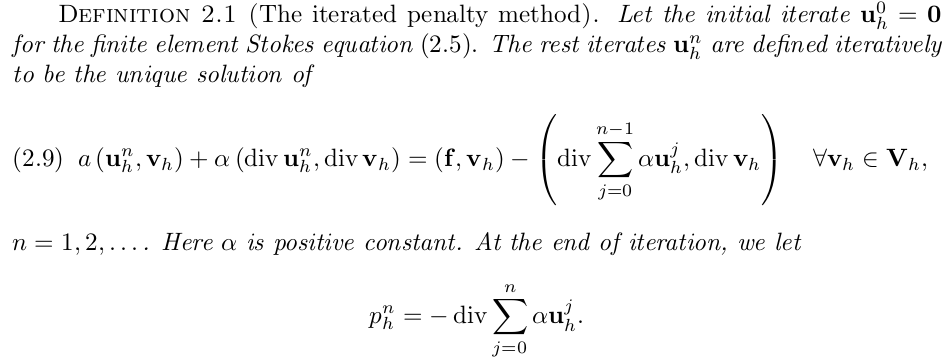
\includegraphics[width=12cm]{python_codes/fieldstone_161/images/iterpen}}
\end{center}

Let us then write the first steps of this algorithm\footnote{For personal reasons
and to establish a parallel with the penalty method, I replace $\alpha$ by $\lambda$.}.
\begin{itemize}
\item
For $n=1$:
\begin{eqnarray}
a({\bm u}_h^1,{\bm v}_h) + \lambda (\text{div}\; {\bm u}_h^1, \text{div}\; {\bm v}_h) 
&=& ({\bm f} , {\bm v}_h) - \text{div}\; \left( \lambda {\bm u}_h^0 , \text{div}\; {\bm v}_h \right) \nn\\
p_h^1 &=& - \text{div}\; [\lambda ( {\bm u}_h^0 + {\bm u}_h^1 )]
\end{eqnarray}
\item 
For $n=2$:
\begin{eqnarray}
a({\bm u}_h^2,{\bm v}_h) + \lambda (\text{div}\; {\bm u}_h^2, \text{div}\; {\bm v}_h) 
&=& ({\bm f} , {\bm v}_h) - \text{div}\; \left( \lambda ({\bm u}_h^0 +{\bm u}_h^1 ), \text{div}\; {\bm v}_h \right) \nn\\
p_h^2 &=& - \text{div}\; [\lambda ( {\bm u}_h^0 + {\bm u}_h^1 + {\bm u}_h^2)]
\end{eqnarray}
\end{itemize}

Concretely, we start with ${\bm u}_h^0={\bm 0}$ and we compute the pressure only when the 
iterations have converged, i.e. the inf norm of the difference between two consecutive 
velocity fields is less than a user chosen tolerance:
\begin{lstlisting}
xi_u=np.max(abs(u_prev-u))/np.max(abs(u))
xi_v=np.max(abs(v_prev-v))/np.max(abs(v))
if xi_u<tol and xi_v<tol:
   break
\end{lstlisting}
These values are written at every iteration in the {\tt conv.ascii} file.

Once the velocity field has been obtained the pressure is computed 
at each corner of each element ($Q_{-1}$ representation).

\newpage
%==========================================
\section*{Grids and dofs}

In \textcite{huzh11} we find the following table:

\begin{center}
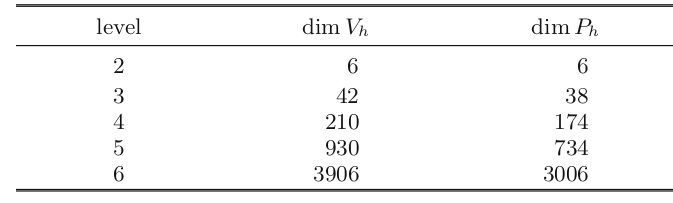
\includegraphics[width=10cm]{python_codes/fieldstone_161/images/dofs}
\end{center}

The authors state that ``The initial grid, level one grid, is simply one unit square''
so that the level 2 grid is a $2\times 2$ element grid:
\begin{verbatim}
+-------+-------+
|       |       |
|       |       |
|       |       |
+-------+-------+
|       |       |
|       |       |
|       |       |
+-------+-------+
\end{verbatim}
with the following velocity dofs:
\begin{verbatim}
u---u---u---u---u   v-------v-------v
|       |       |   |       |       |
|       |       |   v       v       v
|       |       |   |       |       |
u---u---u---u---u   v-------v-------v
|       |       |   |       |       |
|       |       |   v       v       v
|       |       |   |       |       |
u---u---u---u---u   v-------v-------v
\end{verbatim}
Since $u=v=0$ on all boundaries we replace the $u,v$ dofs by $\times$
to indicate that these are no longer degrees of freedom:
\begin{verbatim}
x---x---x---x---x   x-------x-------x
|       |       |   |       |       |
|       |       |   x       v       x
|       |       |   |       |       |
x---u---u---u---x   x-------v-------x
|       |       |   |       |       |
|       |       |   x       v       x
|       |       |   |       |       |
x---x---x---x---x   x-------x-------x
\end{verbatim}
and we indeed find $\text{dim}~V_h=6$. 

\newpage
We consider now a level 3 grid, i.e. $4\times 4$ elements. 
The $u$ dofs are placed as follows:
\begin{verbatim}
u---u---u---u---u---u---u---u---u
|       |       |       |       |
|       |       |       |       |
|       |       |       |       |
u---u---u---u---u---u---u---u---u
|       |       |       |       |
|       |       |       |       |
|       |       |       |       |
u---u---u---u---u---u---u---u---u
|       |       |       |       |
|       |       |       |       |
|       |       |       |       |
u---u---u---u---u---u---u---u---u
|       |       |       |       |
|       |       |       |       |
|       |       |       |       |
u---u---u---u---u---u---u---u---u
\end{verbatim}
After boundary conditions are imposed:
\begin{verbatim}
x---x---x---x---x---x---x---x---x
|       |       |       |       |
|       |       |       |       |
|       |       |       |       |
x---u---u---u---u---u---u---u---x
|       |       |       |       |
|       |       |       |       |
|       |       |       |       |
x---u---u---u---u---u---u---u---x
|       |       |       |       |
|       |       |       |       |
|       |       |       |       |
x---u---u---u---u---u---u---u---x
|       |       |       |       |
|       |       |       |       |
|       |       |       |       |
x---x---x---x---x---x---x---x---x
\end{verbatim}
Only 21 $u$ are left, and we will find as many $v$ dofs, so in this case $\text{dim}(V_h)=21+21=42$,
in accordance with the table. 

Let us now turn to the pressure dofs. 
Warning: it is not as simple as the velocity dofs. 
In \textcite{huzh11} we read: {\color{darkgray} ``we decrease the space $Q_1^{dc}$ 
for the pressure to $Q_1'$, by removing all spurious modes, i.e.,
eliminating one degree of freedom at each vertex. We have to emphasize
that the discrete pressure space is introduced for the analysis, but not in the
computation. By an iterated penalty method, we obtain the discrete solutions
for the pressure without coding the pressure element''}
and in 
\textcite{zhan09}:
{\color{darkgray} ``
We note that, by choosing div($Q_{k+1,k}\times Q_{k,k+1}$) 
as the discrete finite element space for the pressure, the spurious
modes in discontinuous $Q_k$ space are filtered out automatically.
[...]
$P_h$ is a subspace of discontinuous, piecewise polynomials
of separate-degree $k$ or less. As singular vertices are present (see [15, 16]), 
$P_h$ is a proper subset of the discontinuous piecewise $Q_k$ 
polynomials. It is difficult to find a local basis for $P_h$.
[...]
We note that the spurious (checkerboard) modes, generated at each 
singular vertex (cf. (3.8)), in the discrete pressure space are filtered
out naturally.
''}

In \textcite{zhan08} the definition for a singular vertex is given:
\begin{displayquote}
{\color{darkgray}
A vertex is called singular if all edges meeting at the vertex form two cross lines.
}
\end{displayquote}

In order to understand this and arrive at the correct number of pressure dofs
presented in the table above 
it is useful to look at this part of \textcite{huzh11}:

\begin{center}
\fbox{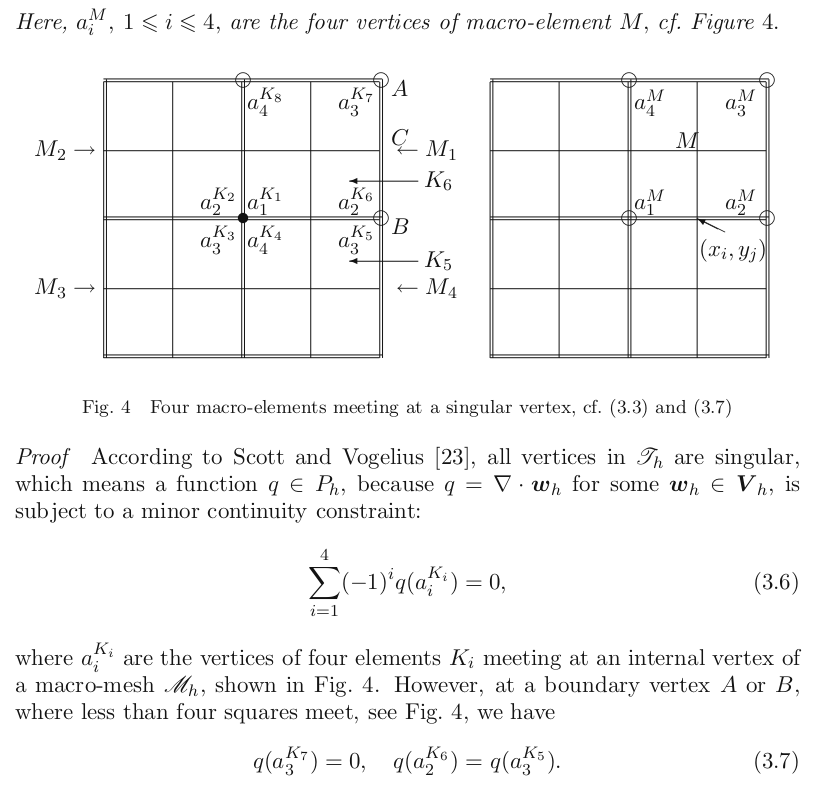
\includegraphics[width=12cm]{python_codes/fieldstone_161/images/pconstraints}}
\end{center}

All nodes are subjected to a constraint. After the mesh is divided 
in $2\times 2$ macro-elements we see that there are 3 type of vertices: the corner ones, 
the mid-edge ones, and the interior ones. 
Let us start with the simplest case: a $2\times 2$ element mesh, i.e. a single macro element.
If the pressure field was a `true' $Q_{-1}$ field\footnote{
Same as $Q_1^{dc}$, but I prefer $Q_{-1}$ to remain consistent 
with the rest of the book.}, we would have 4 pdofs per element,
so $4\cdot 4=16$ pdofs in total:
\begin{verbatim}
+-------+-------+
|4     3|4     3|
|       |       |
|1     2|1     2|
+-------+-------+
|4     3|4     3|
|       |       |
|1     2|1     2|
+-------+-------+
\end{verbatim}
However it is clear from the Eq.~(3.7) above that the corner nodes are constrained to 0, so we
have 4 constraints, i.e. 4 pdofs removed. 
The same equation tells us that mid-edge vertices are constrained (i.e. the pressure 
is continuous at those vertices) so we have again 4 more constraints.
Finally there is one constraint for the vertex in the middle, and one should not 
forget that the pressure space is such that  $\int _\Omega p \; dV=0$, which 
introduces a last constraint. 
In total, 4+4+1+1=10 constraints, so we are left with 16-10=6 pdofs, which is the 
number in the table.

We also find in \textcite{zhmu16}\footnote{That paper is about a different 
FE pair, that is not divergence-free, but it presents the pressure space
of our FE element here.} a rewording of the constraints:
\begin{center}
\fbox{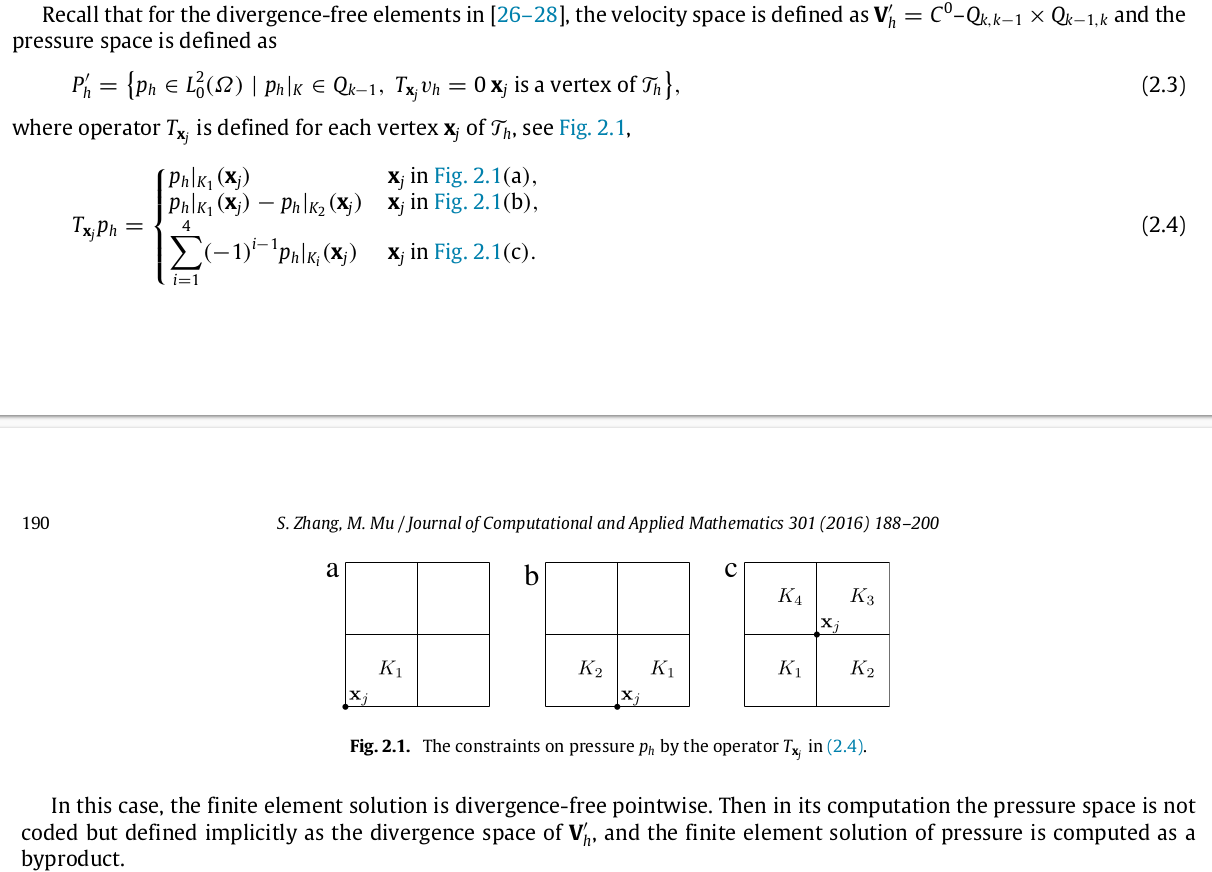
\includegraphics[width=14cm]{python_codes/fieldstone_161/images/zhmu16}}
\end{center}

Let us look at a $4\times 4$ element mesh, i.e. a $2\times 2$ macro element as in the figure above. 
\begin{verbatim}
C-------+-------+-------+-------C
|4     3|4     3|4     3|4     3|
|       |       |       |       |
|1     2|1     2|1     2|1     2|
+-------+-------+-------+-------+
|4     3|4     3|4     3|4     3|
|       |       |       |       |
|1     2|1     2|1     2|1     2|
+-------+-------+-------+-------+
|4     3|4     3|4     3|4     3|
|       |       |       |       |
|1     2|1     2|1     2|1     2|
+-------+-------+-------+-------+
|4     3|4     3|4     3|4     3|
|       |       |       |       |
|1     2|1     2|1     2|1     2|
C-------+-------+-------+-------C
\end{verbatim}
We start from potentially $16\cdot 4=64$ pdofs. We find that 
{\it all} vertices are subjected to a constraint, either because located on a 
corner, an edge or in the middle of four elements. 
This explains the sentence 
{\color{darkgray} ``we decrease the space $Q_1^{dc}$ for the pressure to $Q_1'$, by removing 
all spurious modes, i.e., eliminating one degree of freedom at each vertex.''}
In the end each vertex is assigned a constraint, which removes as many 
pdofs. In this case, $5\cdot 5=25$ constraints. Taking into account the zero-average
constraint, we are left with 64-25-1=38 pdofs, as in the table!

Concretely if the mesh is composed of $n \times n$ elements, then it 
counts $4n^2 - (n+1)^2  -1$ pdofs.
\begin{itemize}
\item $n=2$:  $4n^2 - (n+1)^2 -1= 16 -9 -1=6 $ (we covered that already)
\item $n=4$:  $4n^2 - (n+1)^2 -1= 64 -25 -1=38 $ (we covered that already)
\item $n=8$:  $4n^2 - (n+1)^2 -1= 256 -81 -1=174 $ (value in the table)
\item $n=16$: $4n^2 - (n+1)^2 -1= 1024 -289 -1= 734$ (value in the table)
\end{itemize}

Having understood this, it is clear that it would be very difficult 
to come up with analytical expressions for the pressure basis functions. 

At this stage, we can ask ourselves the question of the consequences of eq(3.7) (i.e. p=0 at corners) 
for generic cases? We shall come back to this later.

Remark: Although the constraints are explained by means of 2x2 macro-elements, 
one could wonder whether using off number of elements per side could yield problems.
I have tried this, and in practice, this makes no difference in the error values nor their 
convergence rates.


%=========================
\section*{code structure}

\begin{verbatim}
build mesh arrays, xu, yu, xv, yv
build connectivity arrays iconu, iconv
define boundary conditions
for iter in range(0,niter):
    build FE matrix and rhs
    solve linear system
    check convergence of u and v fields
compute Q_{-1} pressure and div(v)
compute int p dV
compute divv on markers
compute L2 errors v,p,div(v)
export to paraview
\end{verbatim}
The chosen format for the vtu file is $Q_{-1}$: each element
is exported separately, and 4 corner values for 
each $u$, $v$, $p$, $div(v)$ field.

The {\python bench} parameter allows to choose 
which benchmark is carried out.

All functions are jitted.

Because all elements are rectangles the mapping is trivial
and analytical. 

The following results are obtained by running the basch script
{\tt script\_errors}.

The code relies on a direct solver as provided by scipy.




\newpage
%===============================================
\section*{Manufactured solutions \& experiments}

\subsection*{Huang \& Zhang manufactured solution}

In \textcite{huzh11} (2011) the authors propose the 
following manufactured solution:

\[
g(x,y)=2^8(x-x^2)^2(y-y^2)^2 = 2^8 f(x)h(y) = 256 f(x) h(y)
\]
The velocity is given by 
\[
\vec\upnu 
= 
\left(
\begin{array}{c}
g_y \\ -g_x
\end{array}
\right)
=
\left(
\begin{array}{c}
256 fh' \\
-256 f'h
\end{array}
\right)
%=
%\left(
%\begin{array}{c}
%2^9(x-x^2)^2(1-2y)(y-y^2) \\
%-2^9(1-2x)(x-x^2)(y-y^2)^2 
%\end{array}
%\right)
\]
and the pressure is defined as
\[
p
= -g_{xx}
= -256 f'' h
\]
We have (assuming viscosity is 1) 
\[
\vec{f} = -\Delta \vec{\upnu} + \vec\nabla p
%= 
%\left(
%\begin{array}{c}
%- \Delta g_{y} -g_{xxx}\\
%- \Delta g_{x} -g_{yxx}
%\end{array}
%\right)
%= 
%\left(
%\begin{array}{c}
%- g_{yxx} - g_{yyy} -g_{xxx}\\
%  g_{xxx} + g_{xyy} -g_{yxx}
%\end{array}
%\right)
=256
\left(
\begin{array}{c}
- \Delta (fh') -f''' h  \\
-\Delta (-f'h) -f''h'
\end{array}
\right)
=256
\left(
\begin{array}{c}
- f''h' - fh''' -f''' h  \\
 f'''h + f'h''  -f''h'
\end{array}
\right)
\]
with
\begin{eqnarray}
f(x)&=& (x-x^2)^2 \nn\\
f'(x) &=& 2(1-2x)(x-x^2) \nn\\
f''(x) &=& 2(1-6x+6x^2) \nn\\
f'''(x) &=& 24x-12 \nn
\end{eqnarray}

We have 
\begin{eqnarray}
\iint_\Omega p(x,y) dxdy 
&=& -256 \int_{0}^{1}\int_{0}^{1} f''(x) h(y) dxdy \nn\\
&=& -256 \int_{0}^{1} f''(x) dx \cdot \int_{0}^{1}  h(y) dy \nn\\
&=& -256 \int_{0}^{1} 2(1-6x+6x^2) dx \cdot \int_{0}^{1}  (y-y^2)^2 dy \nn\\
&=& -256 \cdot 0 \cdot \frac{1}{30}  \nn\\ 
&=& 0
\end{eqnarray}
and the pressure is zero at all four corners:
\[
p(0,0)=p(1,1)=p(0,1)=p(1,0)=0
\]


\begin{center}
\fbox{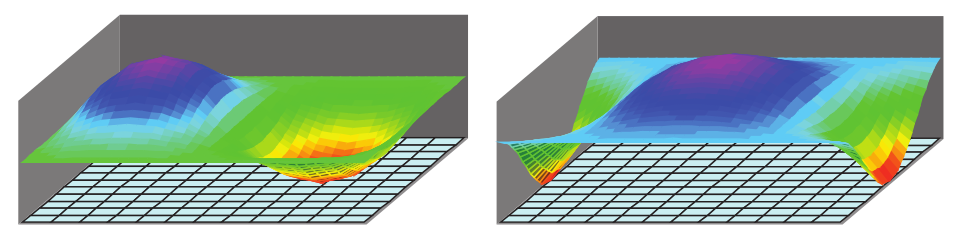
\includegraphics[width=13cm]{python_codes/fieldstone_161/images/mms}}\\
{\captionfont Taken from \cite{zhan09}. Second component of velocity and pressure fields.}
\end{center}

\begin{center}
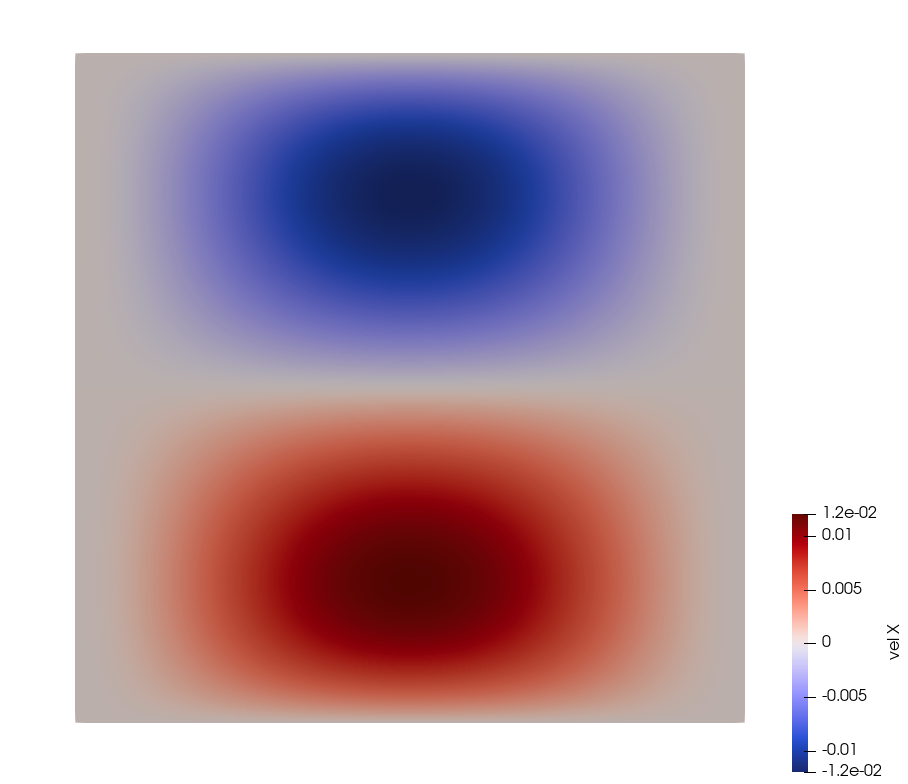
\includegraphics[width=6cm]{python_codes/fieldstone_161/results/bench2/th_u}
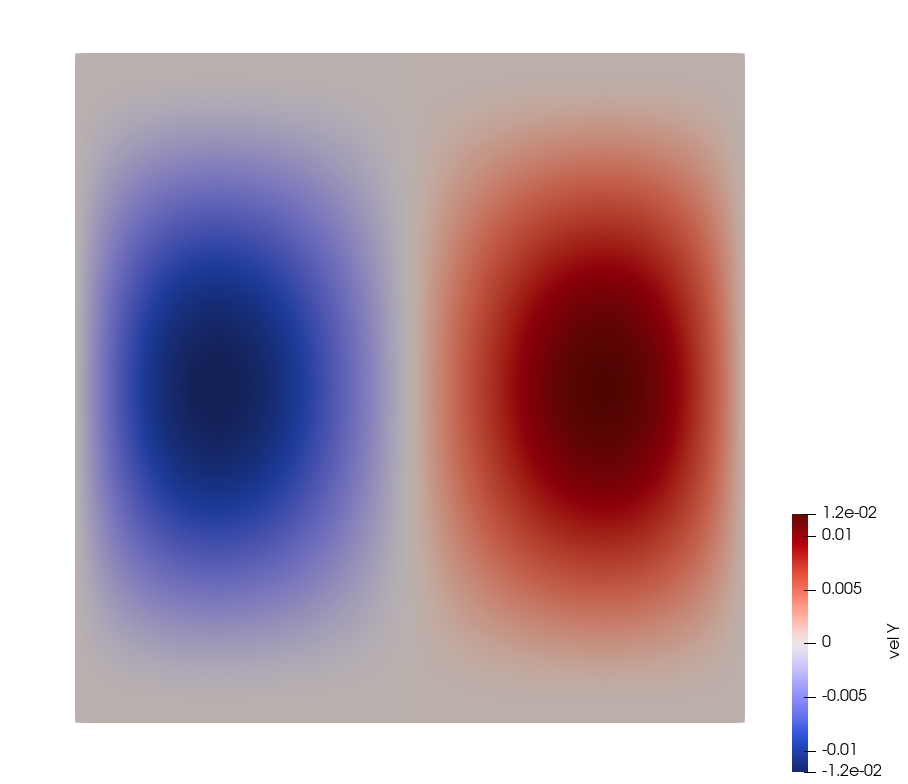
\includegraphics[width=6cm]{python_codes/fieldstone_161/results/bench2/th_v}\\
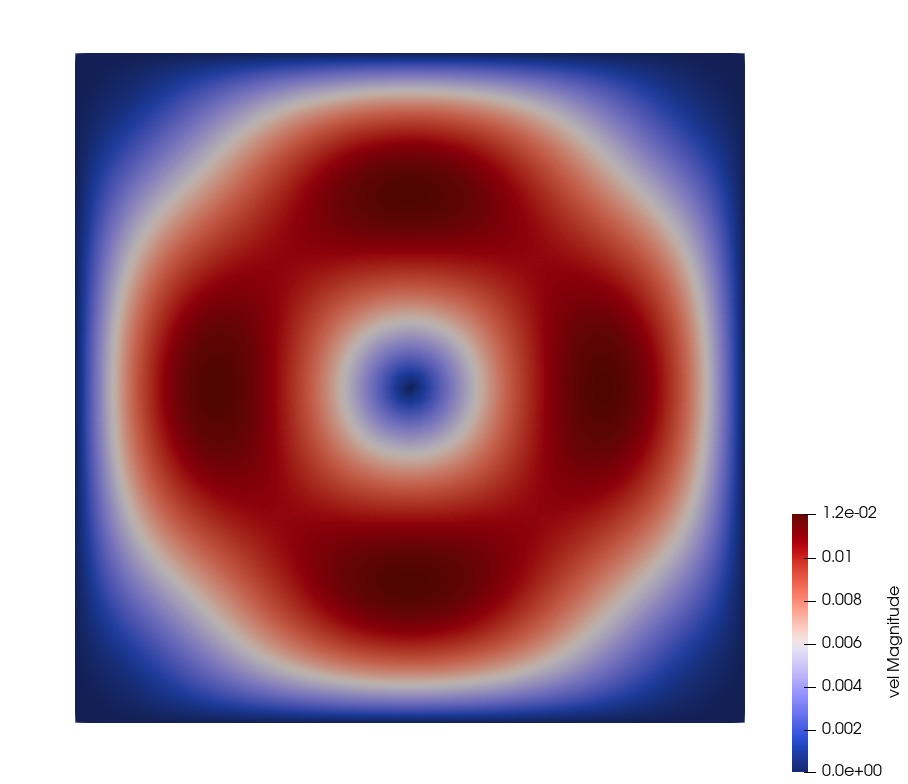
\includegraphics[width=6cm]{python_codes/fieldstone_161/results/bench2/th_vel}
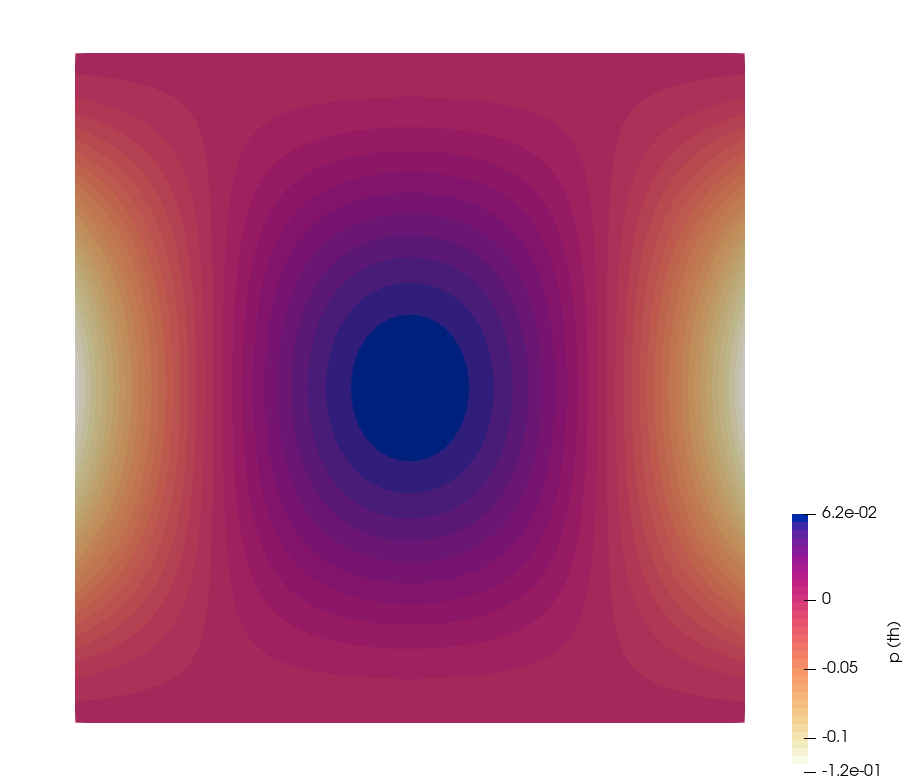
\includegraphics[width=6cm]{python_codes/fieldstone_161/results/bench2/th_press}\\
{\captionfont Figures obtained with Paraview. Visualisation of the analytical solution. 
factor $2^8$ missing.}
\end{center}

They also report the following rates:

\begin{center}
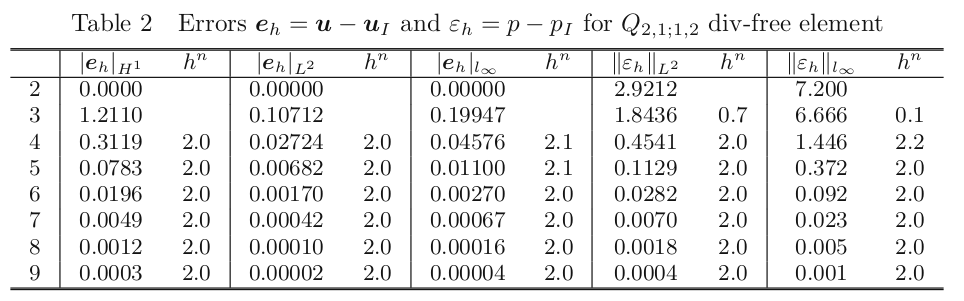
\includegraphics[width=13cm]{python_codes/fieldstone_161/images/errors}
\end{center}

Note that the error convergence rates (in the $L_2$ norm)
are identical for both velocity and pressure. 

%-------------------------------------------------
\subsection*{Donea \& Huerta manufactured solution}

Taken from the Donea \& Huerta book \cite{dohu03}. We consider a two-dimensional problem 
in the square domain $\Omega=[0,1]\times[0,1]$, which possesses a closed-form analytical 
solution. The fluid viscosity is $\eta=1$.
The velocity and pressure fields are given by:
\begin{eqnarray}
u(x,y) 
&=& x^2(1- x)^2 (2y - 6y^2 + 4y^3)  \nn\\
&=& x^2(1-x)^2 2y (1-3y+2y^2) \nonumber\\
&=& x^2(1-x)^2 2y (y-1)(2y-1) \nonumber\\
v(x,y) 
&=& -y^2 (1 - y)^2 (2x - 6x^2 + 4x^3) \nn\\
&=& -y^2 (1 - y)^2 2x (1-3x+2x^2) \nonumber\\
&=& -y^2 (1 - y)^2 2x (x-1)(2x-1) \nonumber\\
p(x,y) &=& x(1 -x)- 1/6 \nonumber 
\end{eqnarray}
Note that the pressure obeys $\int_{\Omega} p \; dV = 0$.

The components of the body force $\vec{b}$ are then
\begin{eqnarray}
b_x &=& (12 - 24y) x^4 + (-24 + 48y) x^3 + (-48y + 72y^2 - 48 y^3 + 12) x^2 \nonumber\\
    && + (-2 + 24y -72y^2+48y^3)x + 1-4y + 12y^2-8y^3 \nonumber\\ 
b_y &=& (8 - 48y + 48 y^2) x^3 + (-12 + 72y - 72y^2) x^2  \nonumber\\
    && + (4 - 24y + 48y^2 - 48y^3 + 24y^4) x - 12y^2 + 24y^3 - 12y^4  \nonumber
\end{eqnarray}

We find that the velocity fields are identical across 
both benchmarks (aside from $2^8$ factor). Only the pressure fields differ!




\newpage
%============================
\section*{Results}

%------------------------------------------------------------ 
\subsection*{Huang \& Zhang manufactured solution ({\tt bench=2})}

The velocity error, pressure error and velocity divergence (in the $L_2$ norm) are 
measured as follows\footnote{$\lambda$ is the penalty parameter.}:  
\begin{center}
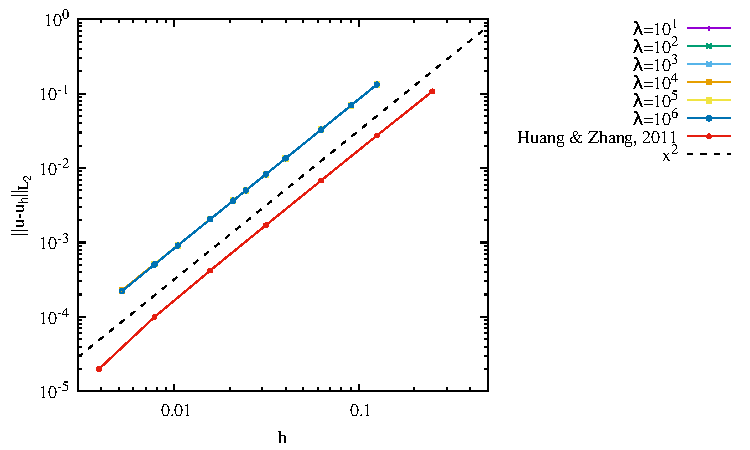
\includegraphics[width=5.7cm]{python_codes/fieldstone_161/results/bench2/errorsV.pdf}
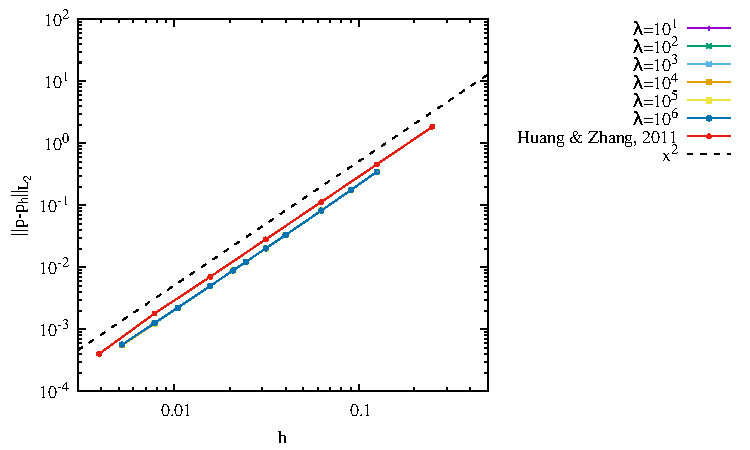
\includegraphics[width=5.7cm]{python_codes/fieldstone_161/results/bench2/errorsP.pdf}
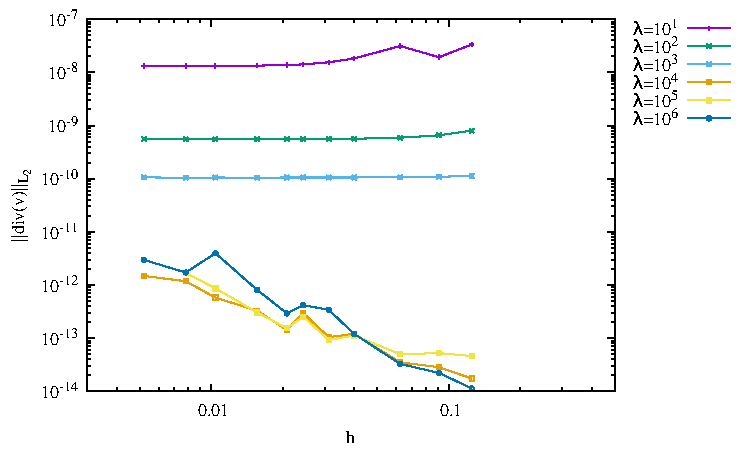
\includegraphics[width=5.7cm]{python_codes/fieldstone_161/results/bench2/errorsDivv.pdf}
\end{center}
As in the publication both velocity and pressure errors converge quadratically.
However there seems to be a factor 5 between my results and theirs for velocity, 
and a factor 1.414 between my results and theirs for pressure. I could 
explain the second by how $h$ is computed (element edge vs. element diagonal), 
but the first one?

On the following plots I show the convergence of the iterated penalty method as 
a function of resolution for different values of the penalty coefficient $\lambda$:

\begin{center}
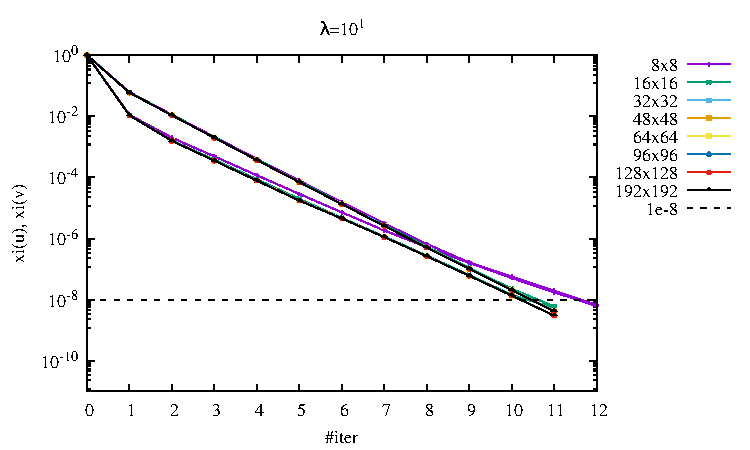
\includegraphics[width=5.6cm]{python_codes/fieldstone_161/results/bench2/conv1.pdf}
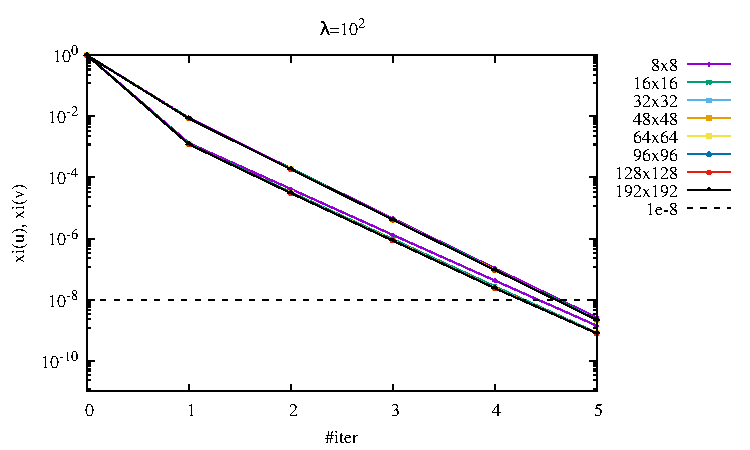
\includegraphics[width=5.6cm]{python_codes/fieldstone_161/results/bench2/conv2.pdf}
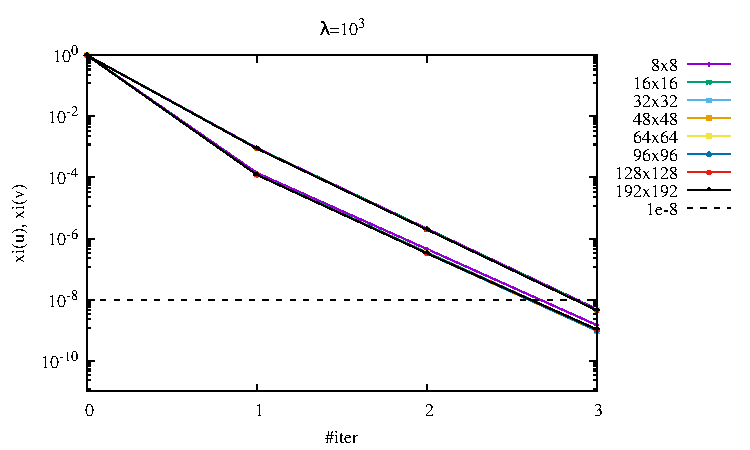
\includegraphics[width=5.6cm]{python_codes/fieldstone_161/results/bench2/conv3.pdf}\\
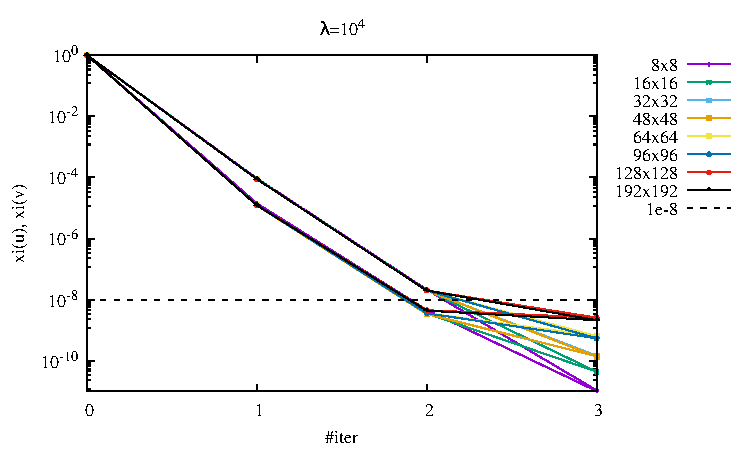
\includegraphics[width=5.6cm]{python_codes/fieldstone_161/results/bench2/conv4.pdf}
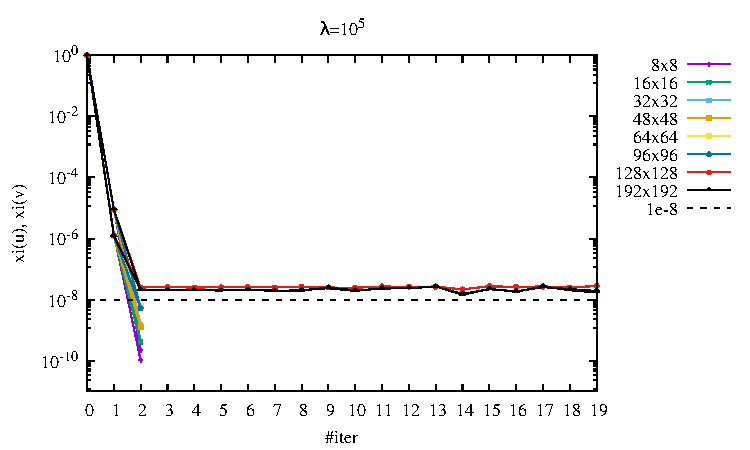
\includegraphics[width=5.6cm]{python_codes/fieldstone_161/results/bench2/conv5.pdf}
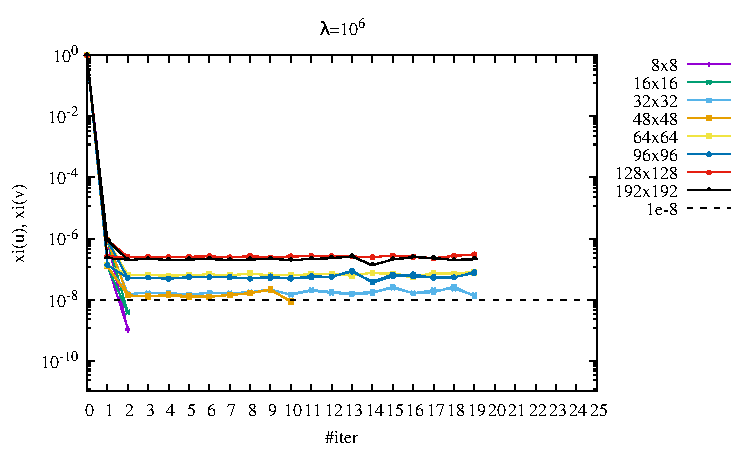
\includegraphics[width=5.6cm]{python_codes/fieldstone_161/results/bench2/conv6.pdf}
\end{center}

Note that at high resolution the cases $\lambda=10^{5}$ and $\lambda=10^6$ fail 
to converge to the desired relative tolerance $10^{-8}$. 

\begin{center}
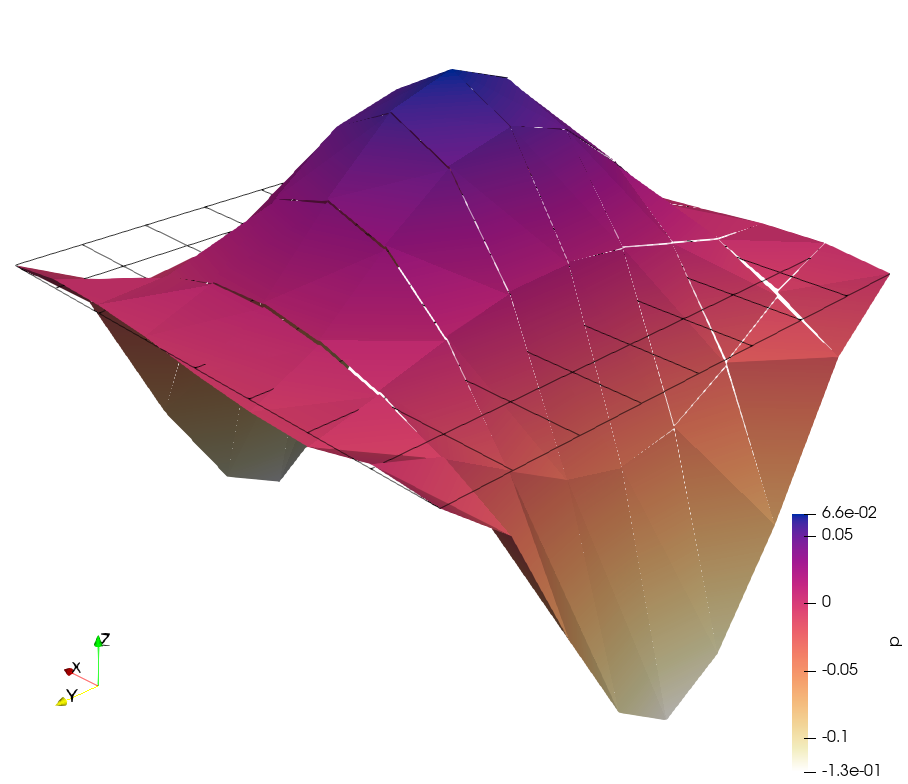
\includegraphics[width=5.7cm]{python_codes/fieldstone_161/results/bench2/press}
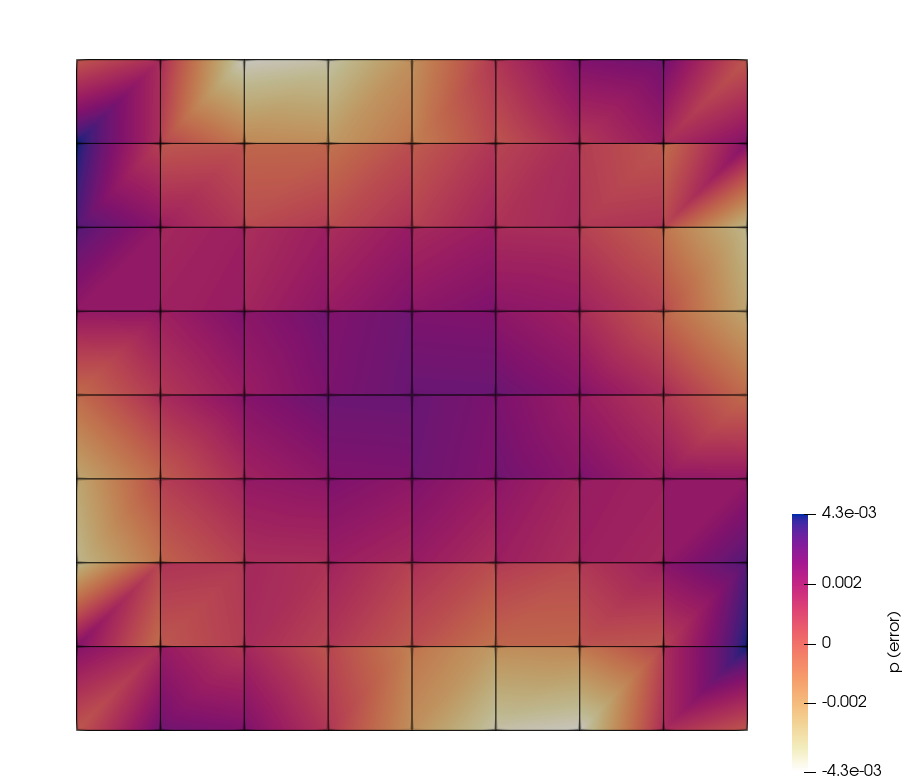
\includegraphics[width=5.7cm]{python_codes/fieldstone_161/results/bench2/press_error}
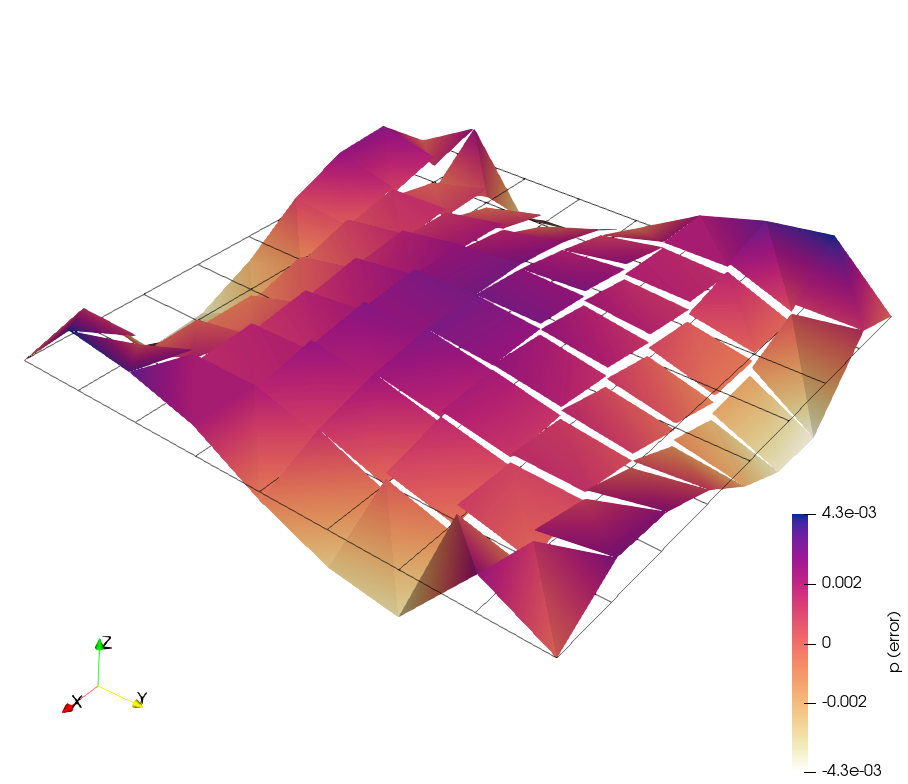
\includegraphics[width=5.7cm]{python_codes/fieldstone_161/results/bench2/press_error2}\\
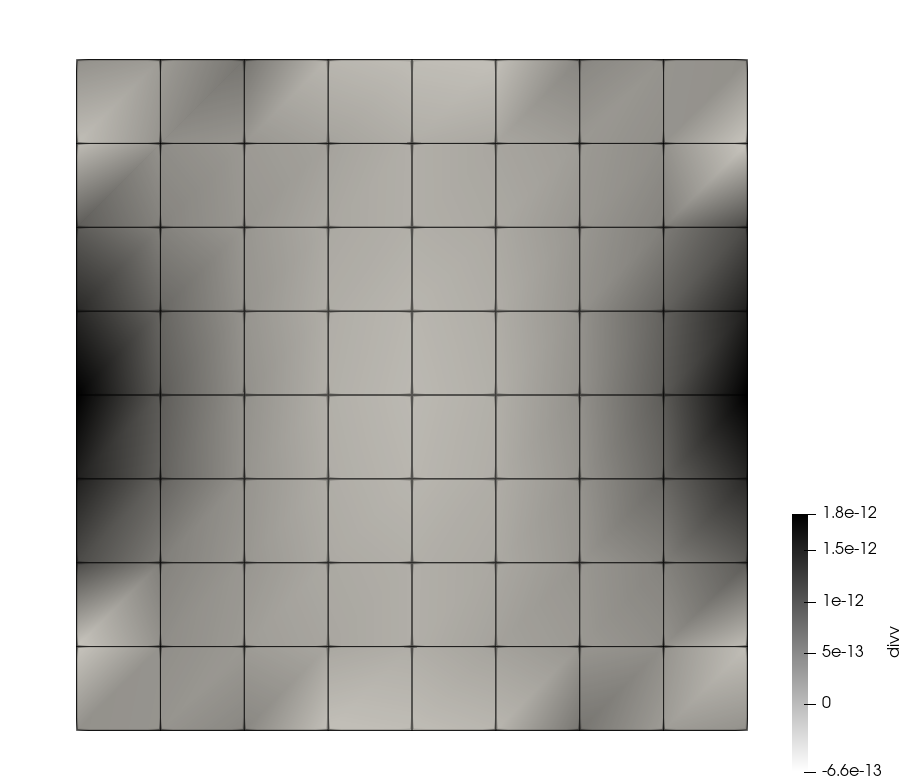
\includegraphics[width=5.7cm]{python_codes/fieldstone_161/results/bench2/divv}
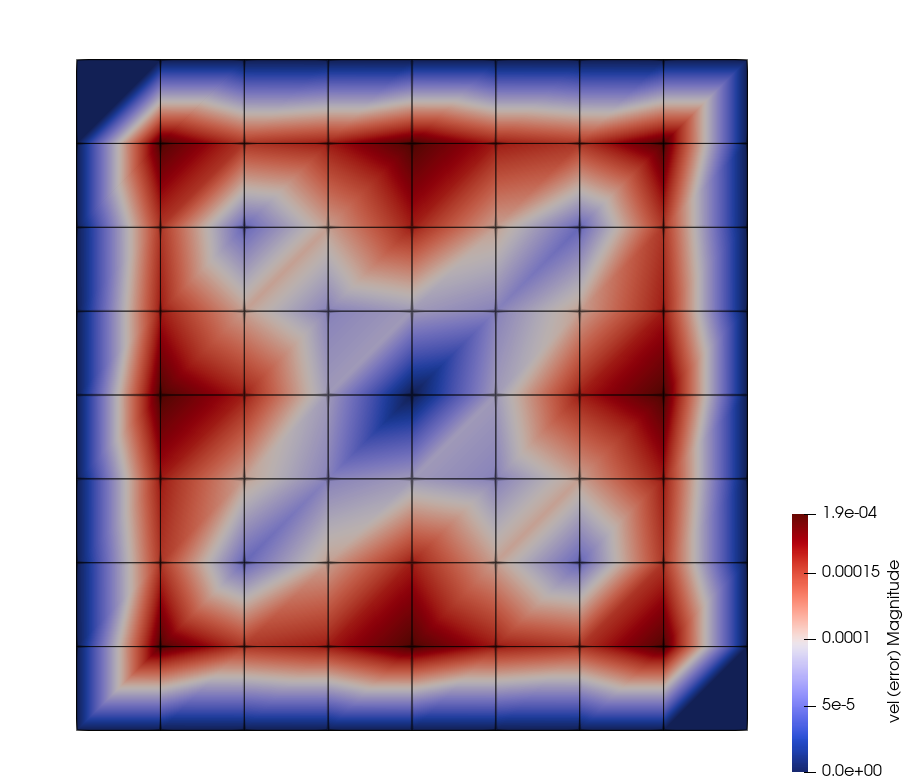
\includegraphics[width=5.7cm]{python_codes/fieldstone_161/results/bench2/vel_error}\\
{\captionfont Obtained on $8\times8$ grid (factor $2^8$ is absent). 
We find that the divergence is indeed very low.
Note that Paraview is misleading: it looks like the squares are divived into 2 triangles but
in reality it is a visualisation artefact!}
\end{center}

It looks like pressure is continuous on the edges of the domain, 
which is indeed what we expect.

After having successfully reproduced the results of \textcite{huzh11}
I now carry out the other manufactured solution.

%------------------------------------------------------------
\subsection*{Donea \& Huerta manufactured solution ({\tt bench=1})}

On the following figures I show the velocity error, pressure error and velocity 
divergence in the $L_2$ norm.
This time the pressure only convergences linearly:

\begin{center}
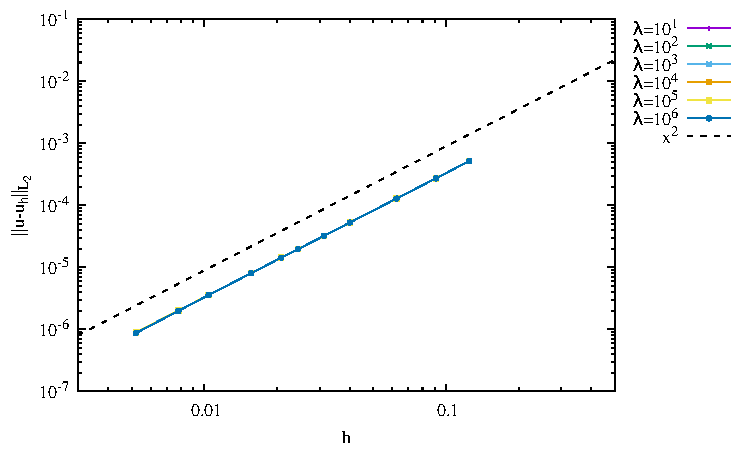
\includegraphics[width=5.7cm]{python_codes/fieldstone_161/results/bench1/errorsV.pdf}
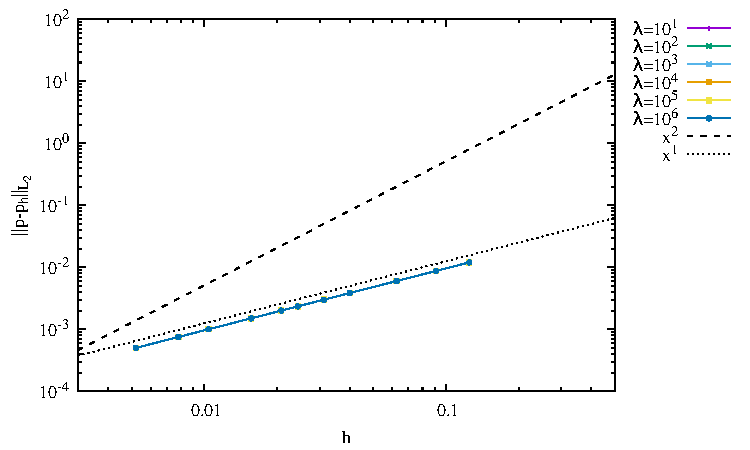
\includegraphics[width=5.7cm]{python_codes/fieldstone_161/results/bench1/errorsP.pdf}
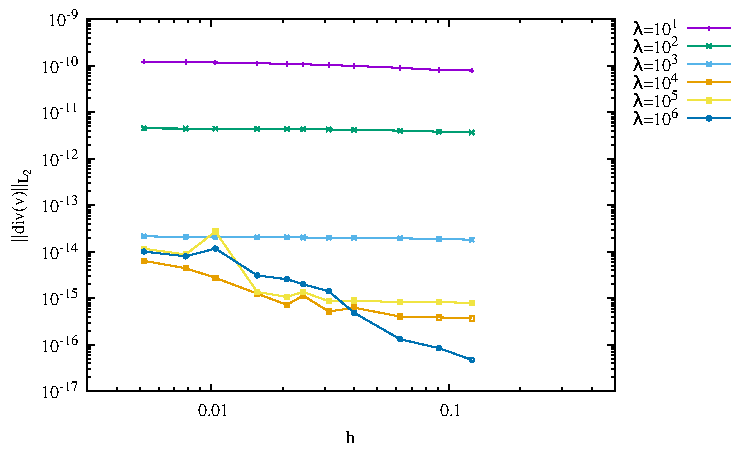
\includegraphics[width=5.7cm]{python_codes/fieldstone_161/results/bench1/errorsDivv.pdf}
\end{center}

We find that the $L_2$ norm of velocity divergence is very low and the higher $\lambda$ the lower 
the divergence.

\begin{center}
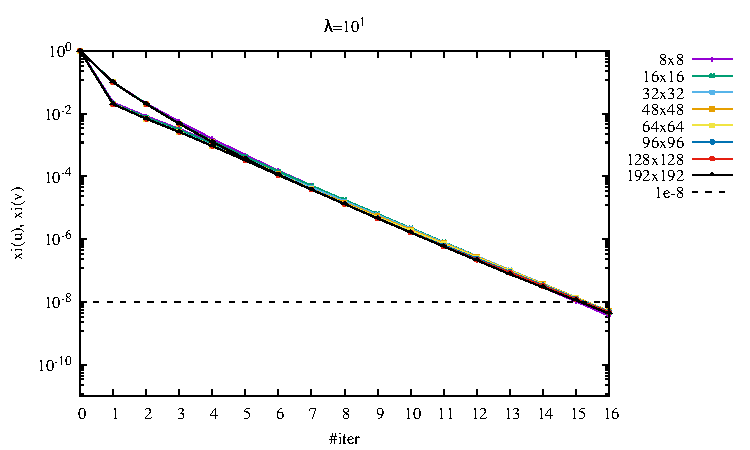
\includegraphics[width=5.7cm]{python_codes/fieldstone_161/results/bench1/conv1.pdf}
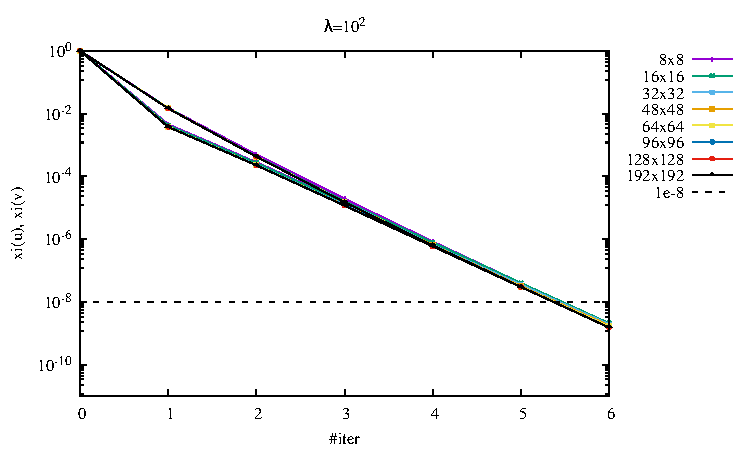
\includegraphics[width=5.7cm]{python_codes/fieldstone_161/results/bench1/conv2.pdf}
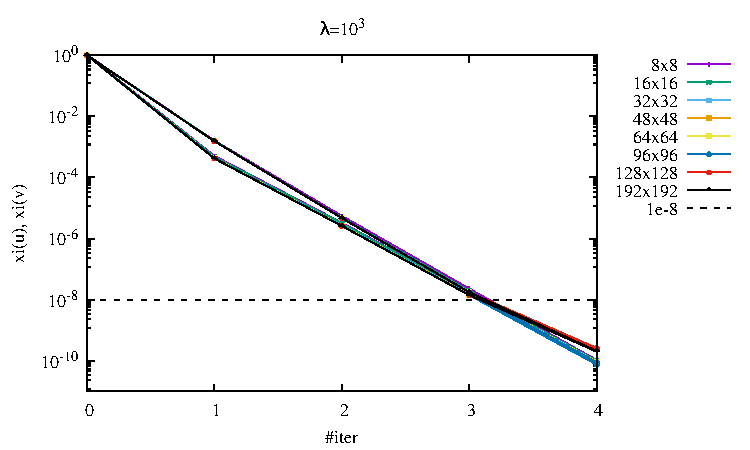
\includegraphics[width=5.7cm]{python_codes/fieldstone_161/results/bench1/conv3.pdf}\\
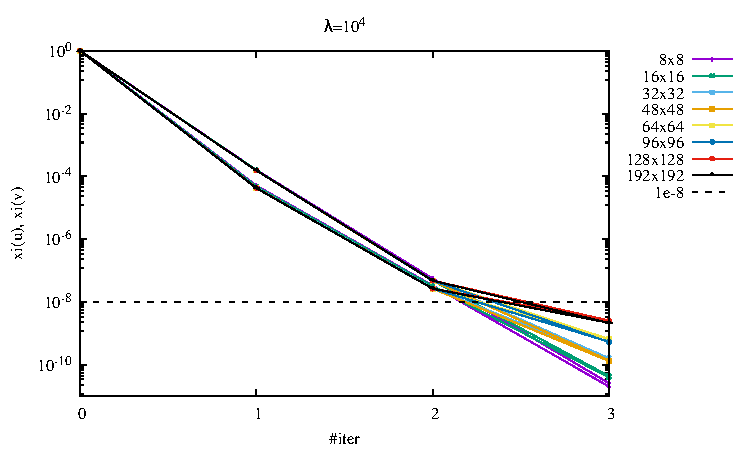
\includegraphics[width=5.7cm]{python_codes/fieldstone_161/results/bench1/conv4.pdf}
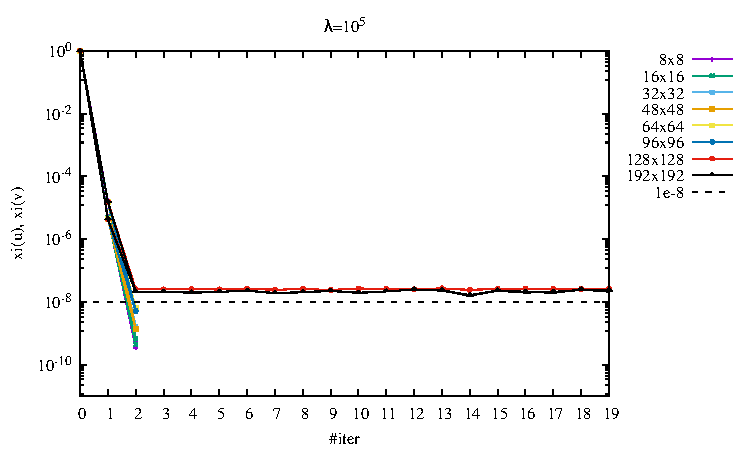
\includegraphics[width=5.7cm]{python_codes/fieldstone_161/results/bench1/conv5.pdf}
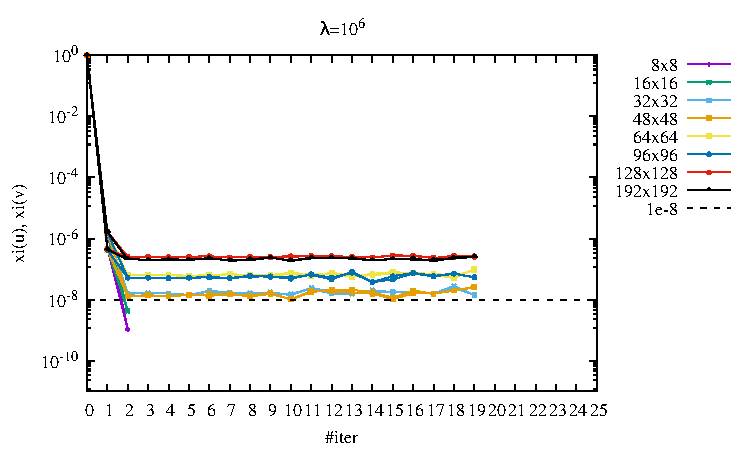
\includegraphics[width=5.7cm]{python_codes/fieldstone_161/results/bench1/conv6.pdf}
\end{center}

We find that for $\lambda \ge 10^2$ the number of iterations becomes really small.
Also the number of iterations to reach convergence decreases when $\lambda$ increases. 
Any value higher than $10^4$ does not improve the convergence, and even worse
at high resolution $\lambda=10^6$ does not converge anymore. 

Let us use a $16\times 16$ mesh with $\lambda=10^3$ and let us look at the error fields, 
i.e. $v_h-v$ and $p_h-p$:
\begin{center}
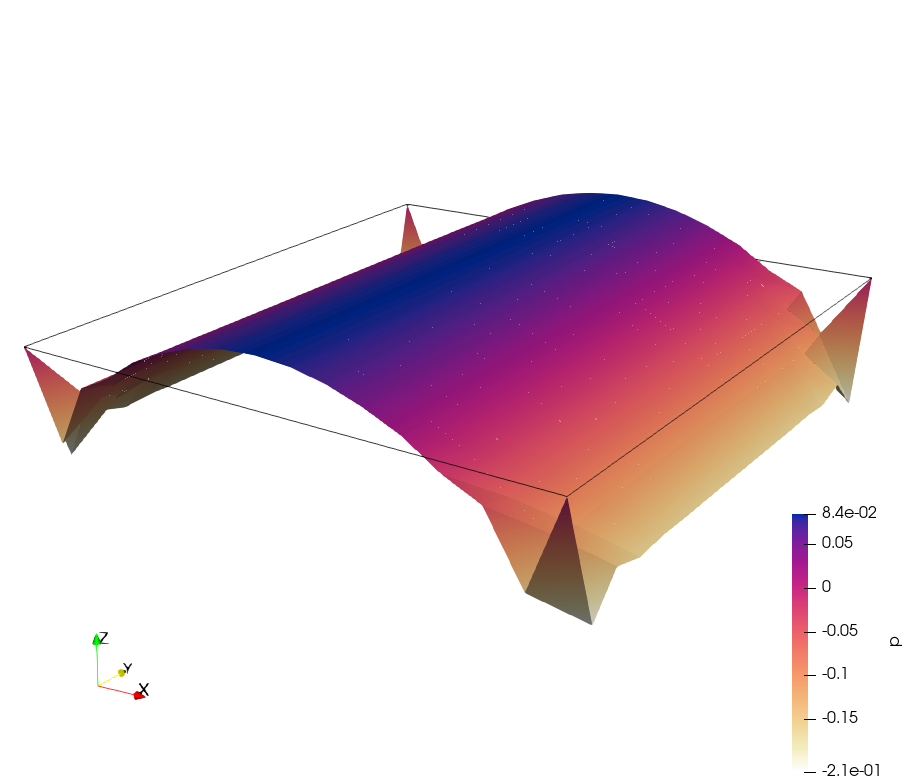
\includegraphics[width=5.7cm]{python_codes/fieldstone_161/results/bench1/press2}
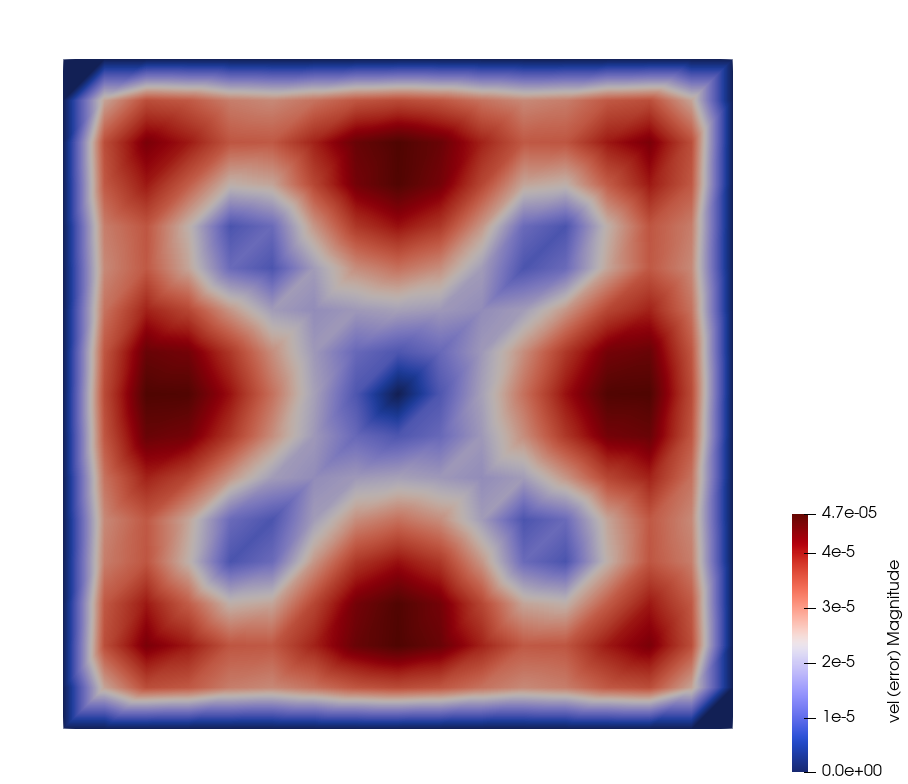
\includegraphics[width=5.7cm]{python_codes/fieldstone_161/results/bench1/vel_error}
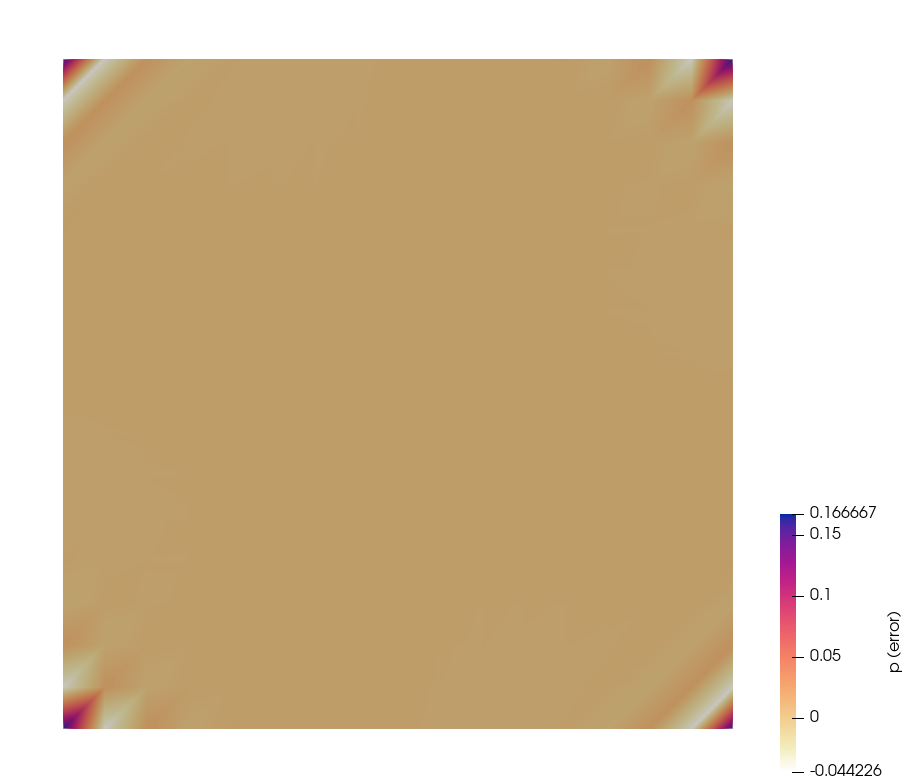
\includegraphics[width=5.7cm]{python_codes/fieldstone_161/results/bench1/press_error}\\
{\captionfont Left: pressure field; Middle: velocity error; Right: pressure error.} 
\end{center}
The analytical pressure field is $p(x,y)=x(1-x)-1/6$. The 1/6=0.16667 term insures that $\int p dV=0$.
We see that the constraints $p=0$ in the corners yield an error that is exactly 1/6 there 
(Everywhere else the error is small, the continuity requirements on the edges do not interfere 
with the true solution). 
This is a big problem that is not discussed in the original paper: is there a way around this?

Remark: after having computed the pressure the code computes the integral of the pressure 
on the domain and the recovered values are extremely small ($<10^{-15}$).  

%------------------------------------------------------------
\subsection*{The sinking block ({\tt bench=3})}

This is a typical test designed to check whether a particular 
FE pair is suitable for buoyancy driven flow (e.g. \textcite{thba22}, 2022).
In this version I keep the viscosity constant in the entire domain with $\eta=1$.
The body force is as follows: in a square of size $0.25\times 0.25$ in the middle of the domain
$\rho \vec{g}=-1.001~\vec{e}_y$ while it is $-1~\vec{e}_y$ outside of it:

\begin{center}
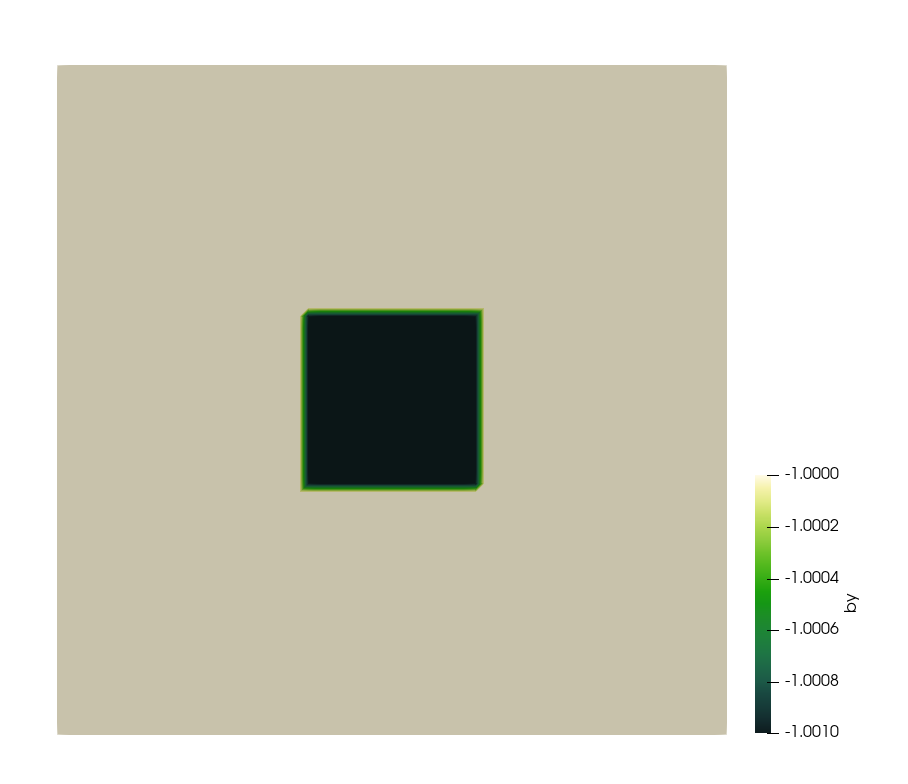
\includegraphics[width=7cm]{python_codes/fieldstone_161/results/bench3/by}\\
{\captionfont Vertical component of the body force. 
It corresponds to a gravity $|\vec{g}|=1$
and a density difference of 0.1\%.}
\end{center}

The reason for choosing this very small density difference is justified by our 
experiments in \textcite{thba22} where it revealed that some FE pairs could not yield 
an accurate velocity solution in the presence of a background hydrostatic pressure
dominating the dynamic pressure. 

The boundary conditions are as follows\footnote{The reasons for this 
peculiar choice will be clear very soon}:
\begin{itemize}
\item Left: no slip
\item Right: free slip
\item Bottom: no slip
\item Top: free slip
\end{itemize}

The solution is as follows (note that this is not a benchmark {\it stricto sensu}
since there is no analytical solution available):

\begin{center}
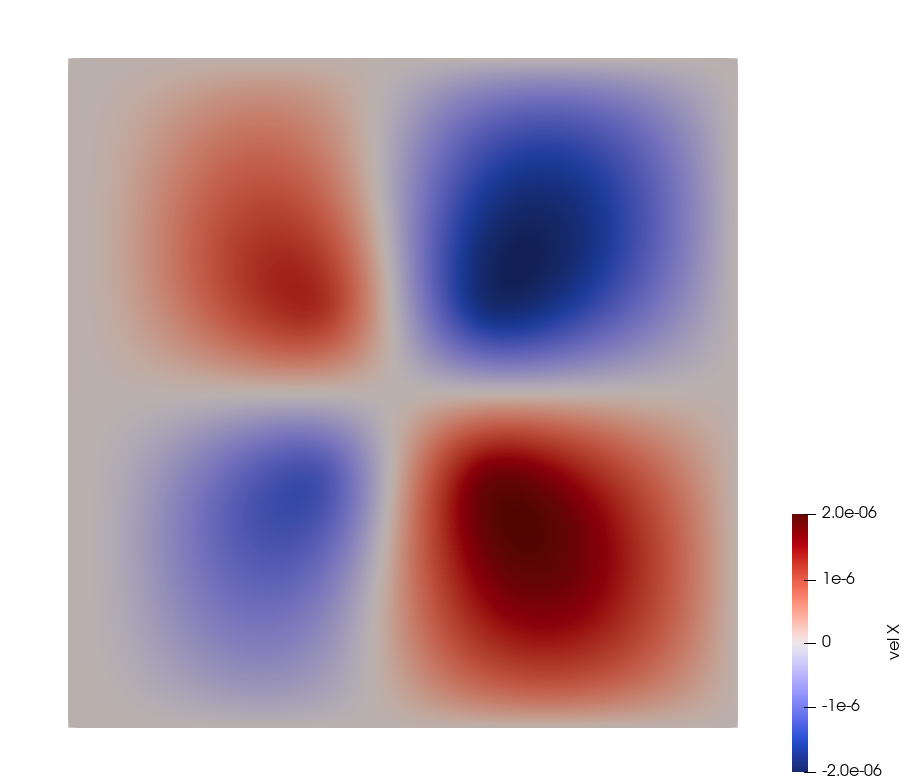
\includegraphics[width=5.7cm]{python_codes/fieldstone_161/results/bench3/u}
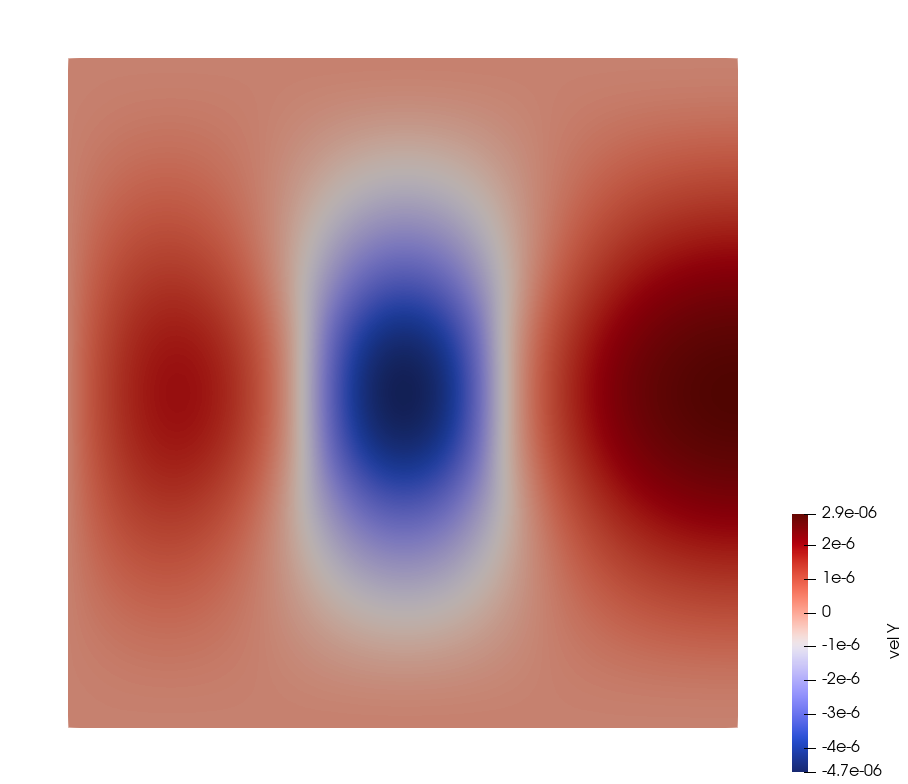
\includegraphics[width=5.7cm]{python_codes/fieldstone_161/results/bench3/v}
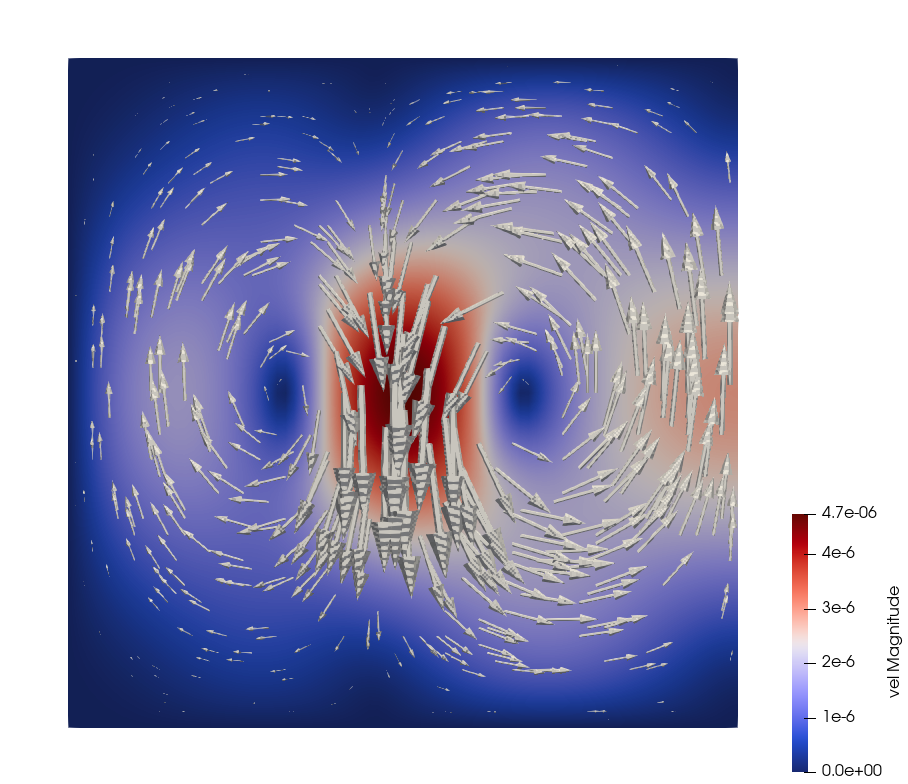
\includegraphics[width=5.7cm]{python_codes/fieldstone_161/results/bench3/vel}\\
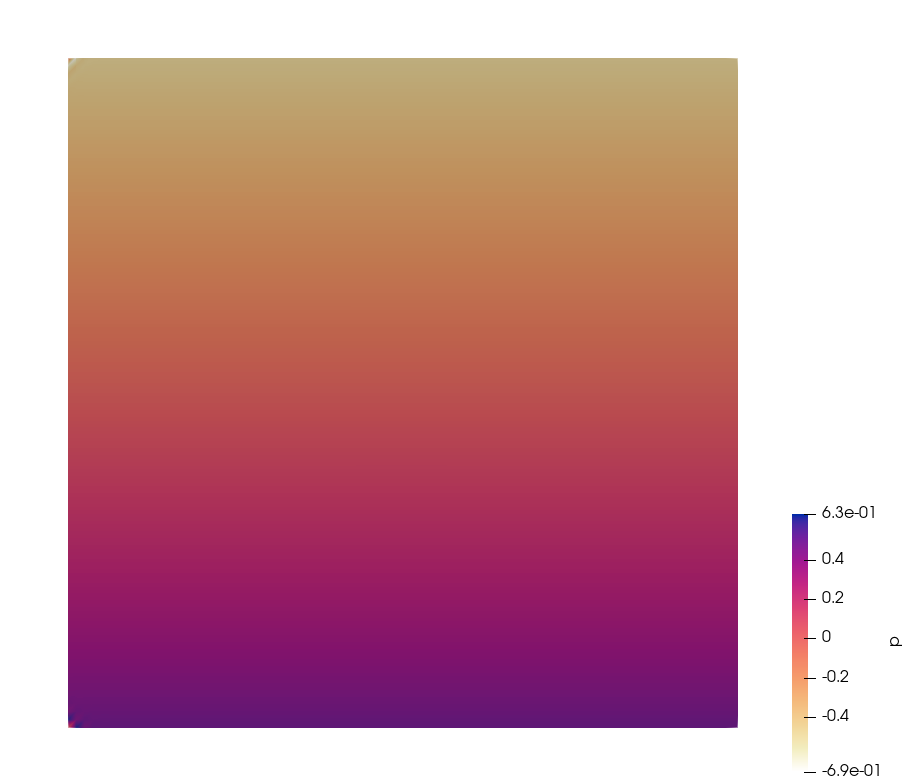
\includegraphics[width=7cm]{python_codes/fieldstone_161/results/bench3/press}
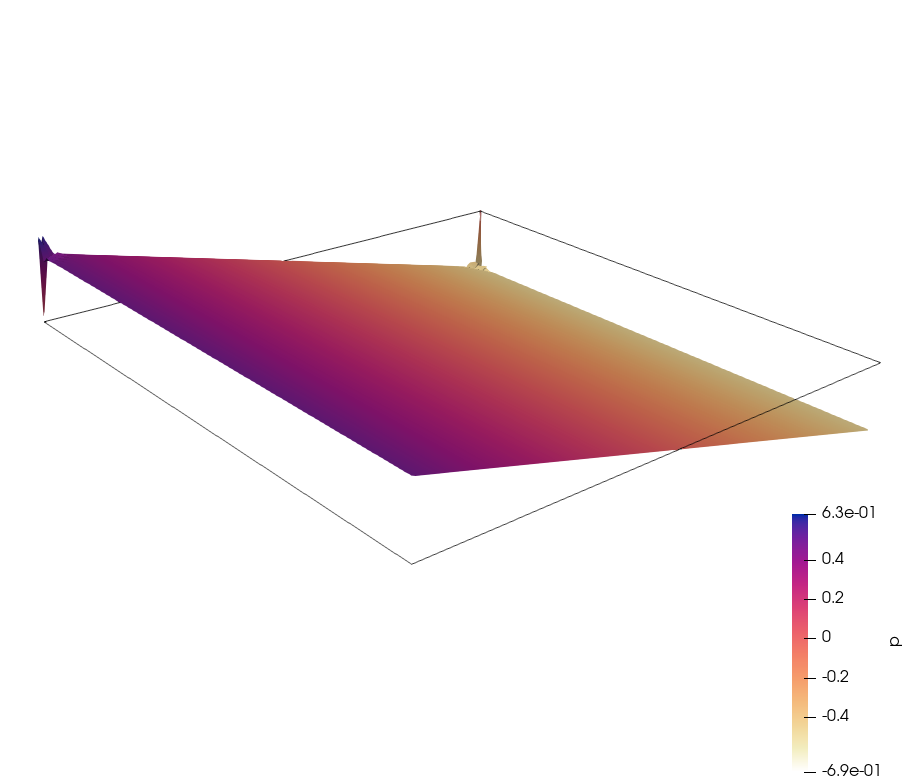
\includegraphics[width=7cm]{python_codes/fieldstone_161/results/bench3/press2}
\end{center}

We find that the velocity field conforms to the boundary conditions and that 
the pressure is (visually) hydrostatic, {\it but} it shows two spikes with abnormal 
values on the top left and bottom left corners (better seen on the right '3d' plot): 
its value is there zero! Rather 
interestingly this happens on the left side, where no-slip boundary 
conditions are prescribed, but not on the right side with free-slip.
This shows the complex interplay between velocity space and the 
constraint $p=0$ at the corners, which casts a shadow on the practical use of this element
in geodynamics where it is common to have no-slip and free-slip boundary conditions on
various sides of the domain.

%------------------------------------------------------------
\subsection*{The viscous inclusion ({\tt bench=4})}

This benchmark originates in \textcite{scpo03} (2003) in which the 
authors derive a simple analytic solution for the pressure and 
velocity fields for a circular 
inclusion under simple shear and it was used 
in \cite{deka08,sunh10,dumg11,krhb12,gemd13}.

\begin{center}
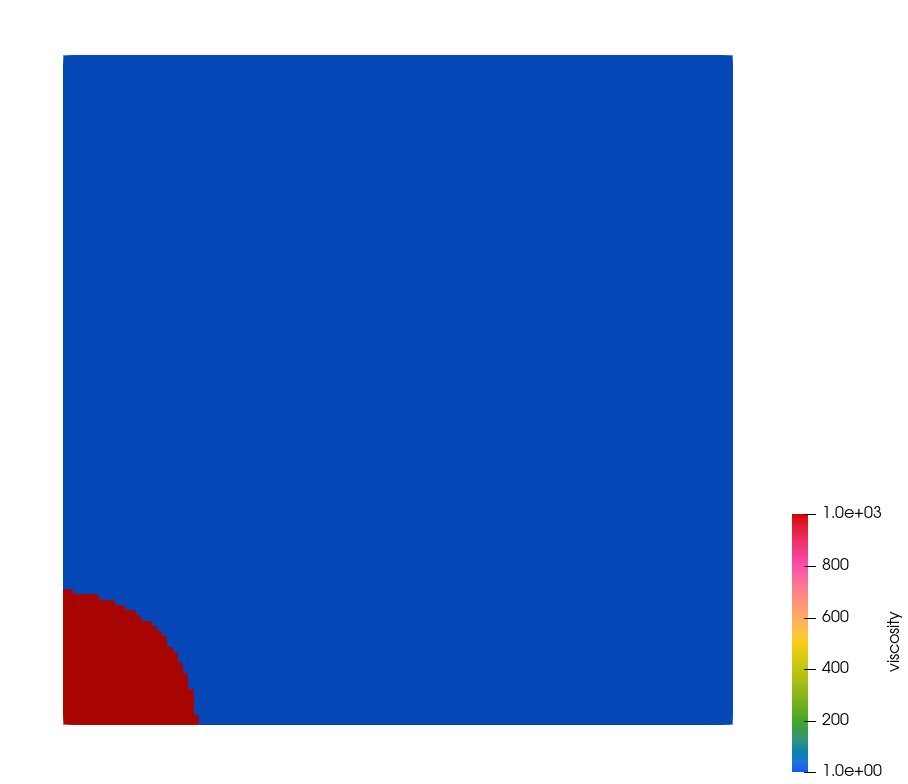
\includegraphics[width=5.7cm]{python_codes/fieldstone_161/results/bench4/eta}
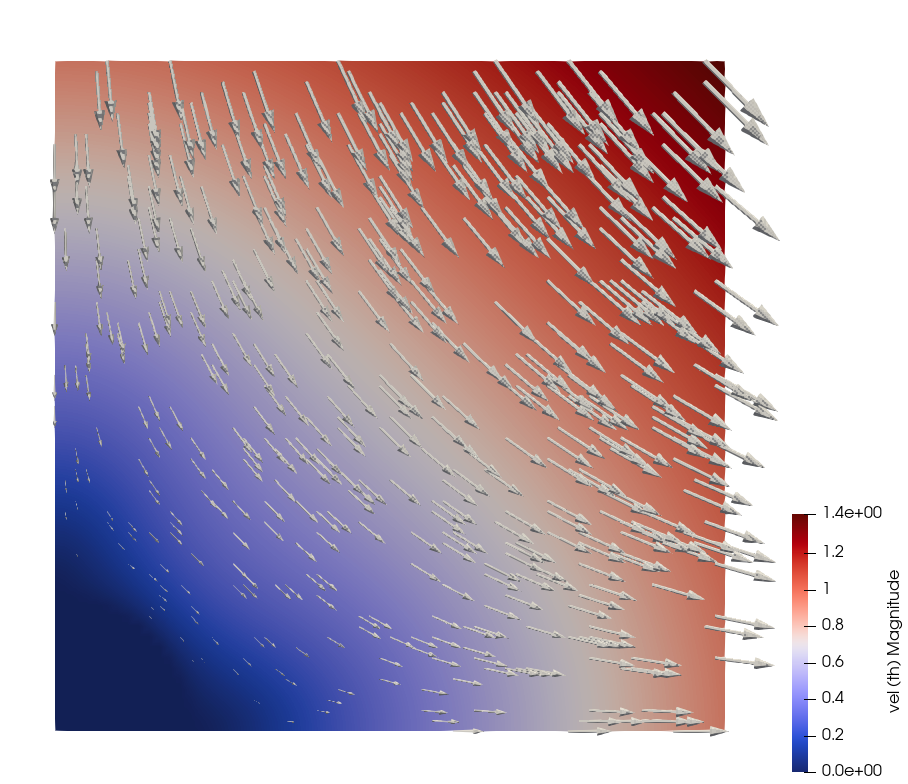
\includegraphics[width=5.7cm]{python_codes/fieldstone_161/results/bench4/vel_th}
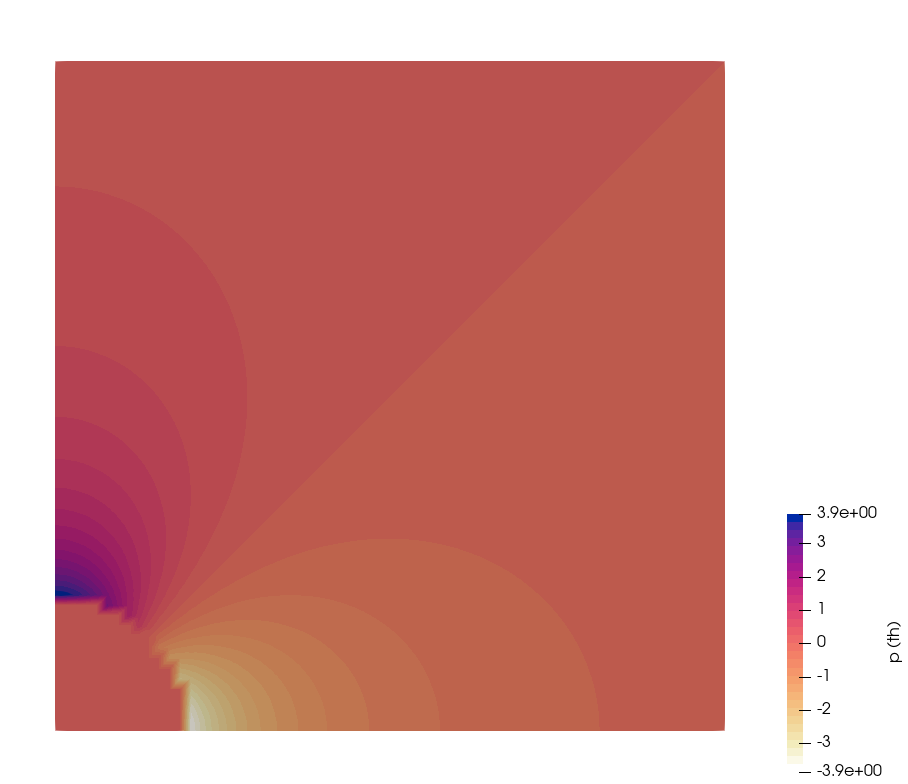
\includegraphics[width=5.7cm]{python_codes/fieldstone_161/results/bench4/press_th}\\
{\captionfont Left: viscosity field on $128\times 128$ mesh; Middle: 
analytical velocity field; Right: analytical pressure field.}
\end{center}

A characteristic of the analytical solution is that the pressure is zero 
inside the inclusion (a circle centered on the origin), while outside it follows the relation
\[
p_m = 4 \dot{\epsilon}
\frac{\eta_m(\eta_i-\eta_m)}{\eta_i+\eta_m}
\frac{r_i^2}{r^2} \cos(2\theta)
\]
where $\eta_i = 10^3$ is the viscosity of the inclusion 
and $\eta_m = 1$ is the viscosity of the background media, $\theta=\tan^{-1}(y/x)$,
and $\dot{\epsilon}=1$ is the applied strain rate.
The velocity expression is too complex to write here (see {\python solution\_solvi}
function in the code).

One important observation with this benchmark is the fact that the 
velocity is not zero even far 
away from the inclusion, so that the analytical (velocity) solution must be imposed on the sides.
Also, because of symmetry, it is often run on the top quadrant $x>0$, $y>0$.

Boundary conditions are free slip on left and bottom boundaries (axes of symmetry)
and the analytical solution is prescribed on the right and top boundaries.
Viscosity is prescribed at the elemental level (i.e. all quadrature points inside an element
are assigned the same viscosity).

\begin{center}
\includegraphics[width=7cm]{python_codes/fieldstone_161/results/bench4/vel}
\includegraphics[width=7cm]{python_codes/fieldstone_161/results/bench4/vel_error}\\
\includegraphics[width=7cm]{python_codes/fieldstone_161/results/bench4/press}
\includegraphics[width=7cm]{python_codes/fieldstone_161/results/bench4/press2}\\
{\captionfont Results obtained on $64\times 64$ grid, $\lambda=10^3$. 
Pressure has been cut off at the analytical min/max for comparison. 
Measured overshoot undershoot are $\pm16$.}
\end{center}

In order for this benchmark to be usable in the context of this element implementation (which 
automatically enforces $\int p \; dV=0$), 
the analytical solution should verify $\int p\; dV=0$. 
In the inclusion $p=0$ so we look at the following integral (the constants have been 
removed for clarity):
\begin{eqnarray}
\int p \; dV \propto \iint \frac{1}{r^2} \cos(2\theta) \; dV 
&=& \iint \frac{1}{r^2} ( \cos^2\theta - \sin^2 \theta) dV \nn\\
&=& \iint \frac{1}{r^2} ( \frac{x^2}{x^2+y^2} - \frac{y^2}{x^2+y^2}) \nn\\
&=& 0
\end{eqnarray}
by symmetry along the diagonal (see also analytical pressure field figure at the 
beginning of this section).
It then makes sense to compute the velocity and pressure error rates:

\begin{center}
\includegraphics[width=5.7cm]{python_codes/fieldstone_161/results/bench4/errorsV.pdf}
\includegraphics[width=5.7cm]{python_codes/fieldstone_161/results/bench4/errorsP.pdf}
\includegraphics[width=5.7cm]{python_codes/fieldstone_161/results/bench4/errorsDivv.pdf}
\end{center}
We recover ${\cal O}(h^1)$ convergence for the velocity error and ${\cal O}(h^{1/2})$ 
pressure error convergence, as in \textcite{thba22} (2022).
Unsurprisingly this element does not (cannot) perform any better than
the ${\bm Q}_2 \times P_{-1}$ element in terms of error rates, since these are
controlled by the fact that the viscosity discontinuity does not align with
element edges.




\newpage
%===============================================
\section*{Discussion/Conclusions/Open questions}

\begin{itemize}

\item The grid/vertex layout is somewhat awkward to build. In practice any naive ordering 
would need re-ordering (reverse Cuthill-Mckee, Sloan, or other) to get a matrix with a reasonable skyline.

\item The pressure space is too complex to build so we {\it have} to use iterative penalty method. 
It seems to converge reasonably nice for $\lambda=10-100$ so this should not 
be too much of a problem for an iterative solver.

\item $Q_{21}\times Q_{12}$ velocity space smaller than than $Q_2\times Q_2$ so the velocity
block smaller for a given number of elements (although it is not spectacular). 
Also, the linear system is as big as the viscosity block, so in case one uses 
a direct solver, cheaper than solving matrix coming from mixed formulation

\item bonus: divergence free element!

\item with Q2Q1, we must iterate (outer solver to arrive at solution, FGMRES, or PCG. 
With this element, outer iterations (iterated penalty method) also necessary. What is best?
\textcite{zhan08} states: `` 
. So it is not possible to find a local basis for Ph in general, and it is not possible to
derive a linear system of equations for (2.6), different from all other mixed finite methods. It
seems that the definition of Ph (2.5) is not practical to implement th mixed element. But
on the other side, it is the special interest of the new formulation where the space Ph is not
implemented at all, and the discrete solutions approximating the pressure function in the Stokes
equations will be obtained as byproducts. So there will be only one finite element space for 
the velocity, and the mixed element pair becomes a single element. This does not only greatly 
simplify the coding work, but also avoids the difficulty of solving non-positive definite systems
of linear equations encountered in the classic mixed element method.
''

\item quid of pressure not zero at corners? write Zhang ? try different mms 

\item matrix does not change during the iterations, this can be exploited in case a direct solver
like MUMPS is used (analysis and factorisation only needed once)!

\item can free surface be envisaged?

\item quid of viscosity constrasts? 

\end{itemize}

Upon my contacting Prof. Zhang, his answer was:
\begin{displayquote}
{\color{darkgray}
 As p is the Lagrange multiplier for enforcing div u=0, then p should be in the divergence space of u.

If $u=0$ on the boundary, then $div u=0$ at boundary corners. 
So, we have to choose the exact solution $p=0$ at corners. 

This way the weak solution in $H^2 \times H^1$ space is the strong solution.

Now if $p \ne 0$ at corners,  one can still find weak solutions in the $H^1 \times L^2$ space.  
But the current element does not produce an optimal order solution for $p$,  
(still the optimal order convergence for u).   $p_h$ converges at 1/2 order or so.

To get an optimal order convergent $p_h$ in this case,  we need to add piecewise polynomial 
bubbles at the corner square elements so that div u is a two piece non-zero constants at each corner.
}
\end{displayquote}

Based on this answer, this concludes my study.  

